\chapter{Controle Baseado em Eventos de Conversores CC-CC} \label{cap4}

% Essa análise fornece insights sobre a aplicação das abordagens de ETC e permite comparar suas vantagens e desvantagens.


\section{Modelo de \acrshort{etm} para Sistemas Lineares} \label{section:etm_models}

% ETM: Apresentação do sistema dinâmico
Nesta pesquisa, é proposto um modelo de \acrshort{etm} dinâmico para sistemas lineares, representada pela equação diferencial abaixo: \begin{equation} \dot{x}(t) = Ax(t) + Bu(t). \label{eq:linear_system_etm}\end{equation} Nesta equação, $ x(t) \in \mathbb{R}^n $ representa o estado do sistema, $ u(t) \in \mathbb{R}^m $ é a entrada de controle, e $ A \in \mathbb{R}^{n \times n} $ e $ B \in \mathbb{R}^{n \times m}$ são a matriz de estados e a matriz de entrada, respectivamente. Além disto, a origem do sistema é considerada o ponto de equilíbrio de interesse.

% ETM: Apresentação do erro de transmissão
Como discutido na seção \ref{section:etm_classification}, quando uma amostra de dados é transmitida no tempo de evento $t_k$, o estado disponível para o controlador é atualizado para $\hat{x}(t) = x(t_k)$, para todo $t$ no intervalo $[t_k, t_{k+1})$. Ao utilizar um \acrshort{zoh}, $\hat{x}(t)$ é mantido constante até o próximo tempo de evento $t_{k+1}$, resultando no erro de transmissão representado por: \begin{equation}
  e(t) = \hat{x}(t) - x(t), \quad \forall t \in [t_k, t_{k+1}).
\end{equation} Este erro ocorre durante o intervalo de tempo entre eventos, $ [t_k, t_{k+1})$.

Desta forma, considerando a seguinte lei de controle por realimentação de estados, ou seja, $u(t) = K\hat{x}(t)$, onde $K \in \mathbb{R}^{1 \times n}$, o sistema linear dinâmico em malha fechada \eqref{eq:linear_system_etm} pode ser expresso pela seguinte equação dinâmica: \begin{gather}
  \dot{x}(t) = Ax(t) + B_u K\hat{x}(t) \notag \\[12pt]
  \dot{x}(t) = Ax(t) + BK[x(t) + e(t)] \notag \\[12pt]
  \dot{x}(t) = (A + BK)x(t) + BKe(t)
  \label{eq:etm_closed_loop}
\end{gather}


% Adicionar um conclusão

\subsection{\acrshort{etm} Estático e Dinâmico}

% Resumo sobre o ETM estático
Conforme apresentado anteriormente, o \acrshort{etm} estático opera considerando apenas os estados atuais do sistema $x(t)$ e o erro de transmissão $e(t)$, e a sua lei de acionamento de eventos é definida como: \begin{equation} t_0 = 0, t_{k+1} = \inf \{t > t_k : \Gamma(x(t), e(t)) < 0 \}, \, \forall k \in \mathbb{N}, \label{eq:static_etm}\end{equation} onde $\Gamma(x, e)$ representa a função de acionamento do \acrshort{etm}. Adicionalmente, para uma classe específica de funções $\Gamma$ dada por \begin{equation}
  \Gamma(x(t), e(t)) = \sigma \alpha(\|x(t)\|) - \beta(\|e(t)\|),
\end{equation} com $\sigma \in (0,1)$, o sistema em malha fechada é assintoticamente estável.

% Função evento proposta
Baseado nisso, é proposta uma condição suficiente para o projeto de um \acrshort{etm} estático e dinâmico usando a abordagem de co-design para o sistema dinâmico linear \eqref{eq:linear_system_etm} controlado por realimentação de estados. Para isso, é considerada uma função de acionamento tal que $\alpha(\|x(t)\|) = x^T(t)\Psi x(t)$, $\beta(\|e(t)\|) = e^T(t)\Xi e(t)$ e $\sigma = 1$, ou seja:  \begin{equation}
  \Gamma(x(t), e(t)) = x^T(t)\Psi x(t) - e^T(t)\Xi e(t),
  \label{eq:etm_gamma}
\end{equation}  onde $\Psi, \, \Xi \in \mathbb{R}^{n \times n}$, e a formulação do seguinte teorema:

\begin{theorem}
  \label{theorem:etm_stability}
  Se existirem matrizes semidefinidas positivas $\Xi, \Psi, X \in \mathbb{R}$ e uma matriz $\tilde{K} \in \mathbb{R}^{m \times n}$ que satisfaçam a seguinte \acrshort{lmi}:
  \begin{equation}
    \begin{bmatrix}
      \mathsf{He}(AX +B\tilde{K}) & B\tilde{K}   & X             \\
      \star                       & -\tilde{\Xi} & 0             \\
      \star                       & \star        & -\tilde{\Psi}
    \end{bmatrix} < 0,
    \label{eq:etm_lmi_1}
  \end{equation}
  então, a origem do sistema em malha fechada é assintoticamente estável com $K = \tilde{K}X^{-1}$, $\Xi= X^{-1}\tilde{\Xi}X^{-1}$, $\Psi = \tilde{\Psi}^{-1}$, $P = X^{-1}$ e a função de Lyapunov definida por $V(x)=x^TPx$.
\end{theorem}

\noindent \textit{Demostração.} Considere que a \acrshort{lmi} \eqref{eq:etm_lmi_1} é factível. Desde que $X$ seja uma matriz semidefinida positiva não singular, esta \acrshort{lmi} pode ser multiplicada por $\mathsf{diag}(X^{-1}, X^{-1}, I)$ no lado esquerdo e direito. Assim, \begin{gather}
  \begin{bmatrix}
    X^{-1} & 0      & 0 \\
    0      & X^{-1} & 0 \\
    0      & 0      & I
  \end{bmatrix}
  \begin{bmatrix}
    \mathsf{He}(AX +B\tilde{K}) & B\tilde{K}   & X             \\
    \star                       & -\tilde{\Xi} & 0             \\
    \star                       & \star        & -\tilde{\Psi}
  \end{bmatrix}
  \begin{bmatrix}
    X^{-1} & 0      & 0 \\
    0      & X^{-1} & 0 \\
    0      & 0      & I
  \end{bmatrix}
  < 0, \notag \notag \\[12pt]
  \begin{bmatrix}
    \mathsf{He}(X^{-1}AX +X^{-1}B\tilde{K}) & X^{-1}B\tilde{K}   & I             \\
    \star                                   & -X^{-1}\tilde{\Xi} & 0             \\
    \star                                   & \star              & -\tilde{\Psi}
  \end{bmatrix}
  \begin{bmatrix}
    X^{-1} & 0      & 0 \\
    \star  & X^{-1} & 0 \\
    \star  & \star  & I
  \end{bmatrix}
  < 0, \notag \notag \\[12pt]
  \begin{bmatrix}
    \mathsf{He}(X^{-1}A +X^{-1}B\tilde{K}X^{-1}) & X^{-1}B\tilde{K}X^{-1}   & I             \\
    \star                                        & -X^{-1}\tilde{\Xi}X^{-1} & 0             \\
    \star                                        & \star                    & -\tilde{\Psi}
  \end{bmatrix}
  < 0,
\end{gather} Como $K = \tilde{K}X^{-1}$, $\Xi= X^{-1}\tilde{\Xi}X^{-1}$, $\Psi = \tilde{\Psi}^{-1}$, $P = X^{-1}$, têm-se: \begin{equation}
  \begin{bmatrix}
    \mathsf{He}(PA +PBK) & PBK   & I             \\
    \star                & -\Xi  & 0             \\
    \star                & \star & -\tilde{\Psi}
  \end{bmatrix} < 0
  \label{eq:inequation_prove}
\end{equation} Por meio do teorema de Schur, a inequação \eqref{eq:inequation_prove} pode ser reescrita como: \begin{equation}
  A_{\mathrm{S}} - B_{\mathrm{S}}D_{\mathrm{S}}^{-1}C_{\mathrm{S}} < 0,
\end{equation} onde, \begin{equation}
  A_{\mathrm{S}} = \begin{bmatrix}
    \mathsf{He}(PA +PBK) & PBK  \\
    (PBK)^T              & -\Xi
  \end{bmatrix}, \,
  B_{\mathrm{S}} = \begin{bmatrix}
    I \\ 0
  \end{bmatrix}, \,
  C_{\mathrm{S}} = \begin{bmatrix}
    I & 0
  \end{bmatrix} \, \mathrm{e} \,
  D_{\mathrm{S}} = -\tilde{\Psi}
\end{equation} Logo, \begin{gather}
  \begin{bmatrix}
    \mathsf{He}(PA +PBK) & PBK  \\
    \star                & -\Xi
  \end{bmatrix} -
  \begin{bmatrix}
    -\tilde{\Psi}^{-1} \\ 0
  \end{bmatrix}
  \begin{bmatrix}
    I & 0
  \end{bmatrix} < 0, \notag \notag \\[12pt]
  \begin{bmatrix}
    \mathsf{He}(PA +PBK) & PBK  \\
    \star                & -\Xi
  \end{bmatrix} -
  \begin{bmatrix}
    -\Psi & 0 \\ 0 & 0
  \end{bmatrix} < 0, \notag \notag \\[12pt]
  \begin{bmatrix}
    \mathsf{He}(PA + PBK) + \Psi & PBK  \\
    \star                        & -\Xi
  \end{bmatrix} < 0
  \label{eq:inequation_prove_2}
\end{gather} Multiplicando a inequação \eqref{eq:inequation_prove_2} por $\begin{bmatrix}
    x^T(t) & e^T(t)
  \end{bmatrix}$ no lado esquerdo, e por $\begin{bmatrix}
    x(t) & e(t)
  \end{bmatrix}^T$ no lado direito, obtém-se: \begin{gather}
  \begin{bmatrix}
    x^T(t) & e^T(t)
  \end{bmatrix}
  \begin{bmatrix}
    \mathsf{He}(PA + PBK) + \Psi & PBK  \\
    \star                        & -\Xi
  \end{bmatrix}
  \begin{bmatrix}
    x(t) \\ e(t)
  \end{bmatrix} < 0 \notag \\[12pt]
  \begin{bmatrix}
    x^T(t) (\mathsf{He}(P(A + BK)) + \Psi) + e^T(t) (PBK)^T &
    x^T(t) PBK - e^T(t) \Xi
  \end{bmatrix}
  \begin{bmatrix}
    x(t) \\ e(t)
  \end{bmatrix} < 0 \notag \\[12pt]
  x^T(t) (\mathsf{He}(P(A + BK)) + \Psi) x(t) + e^T(t) (PBK)^T x(t) +
  x^T(t) PBK e(t) - e(t)^T \Xi e(t)
  < 0 \notag \\[12pt]
  x^T(t) (P\mathsf{He}(A + BK) + \Psi) x(t) + e^T(t) (PBK)^T x(t) +
  x^T(t) PBK e(t) - e(t)^T \Xi e(t)
  < 0 \notag \\[12pt]
  2x^T(t) P[(A + BK)x(t) + BKe(t)] + x^T(t)\Psi x(t) - e^T(t) \Xi e(t)
  < 0
  \label{eq:inequation_prove_3}
\end{gather}  A partir das equações \eqref{eq:linear_system_etm} e \eqref{eq:etm_gamma}, a equação \eqref{eq:inequation_prove_3} pode ser reescrita como: \begin{gather}
  2x^T(t) P\dt{x}(t) + x^T(t)\Psi x(t) - e^T(t) \Xi e(t)  < 0 \notag \\[12pt]
  2x^T(t) P\dt{x}(t) + \Gamma(x(t), e(t)) < 0
  \label{eq:inequation_prove_4}
\end{gather} Como $2x^T(t) P\dt{x}(t) = x^T(t) P\dt{x}(t) + \dt{x}^T(t) P x(t)$ e $\Gamma(x, e) \geq 0, \, \forall t \in [t_k, t_{k+1}), \, \forall k \in \mathbb{N}$ então: \begin{equation}
  x^T(t) P\dt{x}(t) + \dt{x}^T P x(t)  < - \Gamma(x(t), e(t)) < 0.
\end{equation} Logo, \begin{equation}
  x^T(t) P\dt{x}(t) + \dt{x}^T(t) P x(t) < 0.
  \label{eq:final_inequation_prove}
\end{equation} Considerando a função de Lyapunov $V(x) = x^T(t)Px(t)$, a desigualdade \eqref{eq:final_inequation_prove} garante que $\dt{V}(x) < 0$. Portanto, a origem do sistema em malha fechada sob o \acrshort{etm} estático \eqref{eq:static_etm} é assintoticamente estável.

% ETM: Tempo de ocorrência dos eventos e a variável interna dinâmica
No \acrshort{etm} dinâmico, a lei de acionamento de eventos é definida como: \begin{equation} t_0 = 0, t_{k+1} = \inf \{t > t_k : \eta(t) + \theta \Gamma(x(t), e(t)) < 0 \}, \, \forall k \in \mathbb{N} \label{eq:dinamic_etm}\end{equation} onde $\theta \in \mathbb{R}_{\geq 0}$ é um parâmetro de projeto, a função de acionamento $\Gamma(x, e)$ é a mesma definida para o \acrshort{etm} estático, em \eqref{eq:etm_gamma} e $\eta$ é a variável dinâmica definida por: \begin{equation}  \dot{\eta} = - \lambda \eta(t) + \Gamma(x(t), e(t)), \label{eq:eta_dynamic}\end{equation} onde $\lambda \in R_{> 0} $ é o parâmetro de projeto relacionado à taxa de decaimento de $\eta(t)$.

Enquanto o \acrshort{etm} dinâmico não aciona um novo evento, têm-se $\eta(t) + \theta \Gamma(x(t), e(t)) \geq 0$. Se $\theta$ for nulo, então $\eta \geq 0$. Se $\theta$ não for nulo, então \begin{equation}
  \Gamma(x(t), e(t)) \geq - \frac{1}{\theta}\eta(t).
\end{equation} Logo, a partir de \eqref{eq:eta_dynamic},  \begin{equation}
  \dt{\eta}(t) \geq - \left(\lambda + \frac{1}{\theta}\right) \eta(t).
\end{equation} Assim, \begin{equation}
  \eta(t) \geq \eta(0) e ^ {-\left(\lambda + \frac{1}{\theta}\right) t}.
\end{equation} Portanto, $\eta(t) \geq 0$, para todo $t \in [t_k, t_{k+1}), \, \forall k \in \mathbb{N}$. Desta forma, têm-se que $\lambda \eta(t) \geq 0$ e, sob o \autoref{theorem:etm_stability}, a partir da equação \eqref{eq:inequation_prove_4} da demostração apresentada, obtém-se a seguinte inequação para o \acrshort{etm} dinâmico: \begin{gather}
  2x^T(t) P\dt{x}(t) + \Gamma(x(t), e(t)) - \lambda \eta(t) < 0 \notag \\[12pt]
  2x^T(t) P\dt{x}(t) + \dt{\eta}(t) < 0.
\end{gather} Do \autoref{theorem:etm_stability}, foi definido a seguinte função de Lyapunov $V(x) = x^TPx$, logo: \begin{equation}\dt{V}(x) = x^T(t)P\dt{x}(t) + \dt{x}^T(t)Px(t) = 2x^T(t) P\dt{x}(t).\end{equation} Assim, \begin{equation}
  \dt{V}(x) + \dt{\eta}(x) < 0.
\end{equation} Portanto, conforme discutido na seção \ref{section:etm_classification}, para $\dt{W}(x, \eta) = \dt{V}(x) + \dt{\eta}(x) < 0$, a origem do sistema dinâmico \eqref{eq:linear_system_etm} em malha fechada sob o \acrshort{etm} dinâmico baseado no \autoref{theorem:etm_stability} é assintoticamente estável.

Nos \acrshortpl{etm} propostos, a existência de um \acrshort{imee} $\tau$, ou seja, $t_{k+1} - t_k \geq \tau , \, \forall k \in \mathbb{N}$, é fundamental para eliminar o comportamento Zeno, viabilizando, dessa forma, a implementação prática desses \acrshortpl{etm}. Para comprovar a existência do \acrshort{imee} mencionado no \acrshort{etm} estático, inicialmente, considera-se a seguinte inequação derivada da sua lei de acionamento \eqref{eq:static_etm}: \begin{equation}
  \mathcal{G}(x, e) > 1,
\end{equation} onde $\mathcal{G}(x, e) := \displaystyle \frac{e^T\Xi e}{x^T\Psi x}$. Quando um novo evento é acionado, isto é, $t = t_k$, o erro $e(t)$  e $\mathcal{G}(x, e)$ são nulos. Por outro lado, enquanto um novo evento não é acionado, tém-se $0 < \mathcal{G}(x, e) < 1$. Considerando que \begin{equation} \mathcal{G}(x, e) \leq \Lambda \left(\frac{\|e(t)\|}{\|x(t)\|}\right) ^ 2, \end{equation} onde $\Lambda = \displaystyle \frac{\lambda_{\max}(\Xi)}{\lambda_{\min}(\Psi)}$, nenhum evento é acionado enquanto \begin{equation}
  \frac{\|e(t)\|}{\|x(t)\|} \leq \frac{1}{\sqrt{\Lambda}}.
\end{equation} Seja a dinâmica de $\displaystyle \frac{\|e(t)\|}{\|x(t)\|}$ definida como: \begin{gather}
  \frac{\mathrm{d}}{\mathrm{d}t}\left(\frac{\|e(t)\|}{\|x(t)\|}\right) = - \frac{e^T\dt{x}(t)}{\|e(t)\|\|x(t)\|} - \frac{x^T\dt{x}(t) \|e(t)\|}{\|x(t)\|^2 \|x(t)\|} \notag \\[12pt]
  \frac{\mathrm{d}}{\mathrm{d}t}\left(\frac{\|e(t)\|}{\|x(t)\|}\right) \leq - \frac{\|e(t)\|\|\dt{x}(t)\|}{\|e(t)\|\|x(t)\|} - \frac{\|x(t)\| \|\dt{x}(t)\| \|e(t)\|}{\|x(t)\|^2 \|x(t)\|} \notag \\[12pt]
  \frac{\mathrm{d}}{\mathrm{d}t}\left(\frac{\|e(t)\|}{\|x(t)\|}\right) \leq \left( 1 + \frac{\|e(t)\|}{\|x(t)\|} \right) \frac{\|\dt{x}(t)\|}{\|x(t)\|}.
  \label{eq:imee_inequation_1}
\end{gather} Além disso, a partir do sistema em malha fechada \eqref{eq:etm_closed_loop}, é possível definir uma constante $L \in \mathbb{R}_{>0}$ tal que: \begin{gather}
  \|\dt{x}(t)\| = \| (A + BK) x(t) + BKe(t) \| \notag \\[12pt]
  \|\dt{x}(t)\| \leq L(\|x(t)\| + \|e(t)\|)
  \label{eq:imee_inequation_2}.
\end{gather} Desta forma, das inequações \eqref{eq:imee_inequation_1} e \eqref{eq:imee_inequation_2}, tém-se: \begin{gather}
  \frac{\|\dt{x}(t)\|}{\|x(t)\|} \leq L\left(1 + \frac{\|e(t)\|}{\|x(t)\|}\right) \notag \\[12pt]
  \left( 1 + \frac{\|e(t)\|}{\|x(t)\|} \right) \frac{\|\dt{x}(t)\|}{\|x(t)\|} \leq L\left( 1 + \frac{\|e(t)\|}{\|x(t)\|} \right) ^ 2 \notag \\[12pt]
  \frac{\mathrm{d}}{\mathrm{d}t}\left(\frac{\|e(t)\|}{\|x(t)\|}\right) \leq L\left( 1 + \frac{\|e(t)\|}{\|x(t)\|} \right) ^ 2.
  \label{eq:imee_inequation_3}
\end{gather} Definindo $\varphi (t) = \displaystyle \frac{\|e(t)\|}{\|x(t)\|}$, a inequação \eqref{eq:imee_inequation_3} pode ser reescrita como: \begin{equation}
  \dt{\varphi}(t) \leq L \left(1 + \varphi(t)\right)^2.
\end{equation} Desta forma, é possível concluir que $\varphi(t) \leq \psi(t, \psi_0)$, onde $\psi(t, \psi_0)$ é o valor inicial de $\dt{\psi} = L(1 + \psi(t))^2$, com $\psi(0, \psi_0) = \psi_0$. Como $\mathcal{G}(x, e) > 1$, $\psi(t, 0)$ evolui de 0 a $\frac{1}{\sqrt{\Lambda}}$ e, portanto, leva mais tempo para evolui de 0 a 1, do que $\psi(t, 0)$ alcançar $\frac{1}{\sqrt{\Lambda}}$. Portanto, o tempo entre eventos são limitados pelo tempo que $\psi$ leva para evoluir de 0 a $\frac{1}{\sqrt{\Lambda}}$, o que significa que o tempo entre eventos são limitados pela solução $\tau \in \mathbb{R}_{>0}$ de $\psi(\tau, 0) = \frac{1}{\sqrt{\Lambda}}$. Como $\psi(\tau, 0) = \frac{\tau L}{1 - \tau L}$, então o \acrshort{imee} $\tau$ do \acrshort{etm} estático é definido por: \begin{gather}
  % \frac{1}{\sqrt{\Lambda}} = \frac{\tau L}{1 - \tau L} \\[12pt]
  % 1 - \tau L = \tau L \sqrt{\Lambda} \\[12pt]
  % \tau L (1 + \sqrt{\Lambda}) = 1 \\[12pt]
  \tau = \frac{1}{L(\sqrt{\Lambda} + 1)}.
  \label{eq:imee_final_inequation}
\end{gather} Além disto, sob mesmas condições iniciais, o \acrshort{imee} do \acrshort{etm} dinâmico é maior ou igual ao \acrshort{imee} do \acrshort{etm} estático, e portanto, há a exclusão do comportamento Zeno.

% ETM: Condições de Co-design
\subsection{Minimização do número de eventos}

Por meio do \acrshort{imee} $\tau$ definido na equação \eqref{eq:imee_final_inequation}, pode-se observar que \acrshort{imee} apresenta uma relação inversa a $\Lambda$, definida como: \begin{equation}
  \Lambda = \frac{\lambda_{\max}(\Xi)}{\lambda_{\min}(\Psi)}
\end{equation} Desta forma, para reduzir o número de eventos gerados, pode-se aumentar o valor de \acrshort{imee} por meio da minimização de $\Lambda$. Para isto, é necessário minimizar $\lambda_{\max} (\Xi)$ e maximizar $\lambda_{\min}(\Psi)$. Como $\Xi = X^{-1}\tilde{\Xi}X^{-1}$ e $\Psi = \tilde{\Psi}^{-1}$, para minimizar $\lambda_{\max} (\Xi)$ e maximizar $\lambda_{\min}(\Psi)$, os autovalores de $\tilde{\Xi}$ e $\tilde{\Psi}$ precisam ser minimizados.

Portanto, é proposto o seguinte problema de otimização que visa minimizar $\lambda_{\max} (\Xi)$ e maximizar $\lambda_{\min}(\Psi)$: \begin{gather}\underset{X, \tilde{\Xi}, \tilde{\Psi}, \tilde{K}}\min \quad \mathrm{tr}(\tilde{\Xi} + \tilde{\Psi}). \\ \textrm{sujeito a \acrshort{lmi} } \eqref{eq:etm_lmi_1} \label{eq:optimization_problem}\end{gather} A solução deste problema tende a minimizar os autovalores de $\tilde{\Xi}$ e $\tilde{\Psi}$ e a aumentar o intervalo de tempo entre os eventos. Se o problema for factível, é possível determinar as variáveis do problema e obter os parâmetros de projeto do \acrshort{etm} capazes de reduzir o número de transmissões geradas pelo \acrshort{etm}.

\section{Conversores em Malha Fechada sob \acrshort{etm} Estático}

Esta seção aborda a análise dos conversores Buck e Boost em malha fechada sob o \acrshort{etm} estático, os quais foram previamente analisados em malha aberta na Seção \ref{section:open_loop}. Os ETMs foram projetados visando minimizar o número de eventos, utilizando a abordagem por co-design proposta e discutida na seção anterior, \autoref{section:etm_models}.

Para cada simulação, são apresentados o sinal de entrada duty cycle $d(t)$ determinado pelo controlador  e os estados dos conversores: a corrente do indutor $i_L(t)$ e a tensão do capacitor $v_C(t)$. O intervalo entre eventos (\acrshort{itee}) é calculado como a diferença de tempo entre o acionamento de eventos consecutivos, representado por $\Delta_{\acrshort{itee}} = t_{k + 1} - t_k, \, k \in \mathbb{N}$.

Para avaliar o desempenho, são obtidos e apresentados diversos parâmetros, tais como o valor médio dos \acrshortpl{itee} de cada simulação, os tempos de acomodação, a \acrfull{ise}, a \acrfull{itse} e a \acrfull{isc}. Tais integrais são definidas a seguir: \begin{gather}
  \acrshort{ise} = \int_0^{t_\mathrm{s}} e^2(t) \, \mathrm{d}t \\[12pt]
  \acrshort{itse} = \int_0^{t_\mathrm{s}} t e^2(t) \, \mathrm{d}t \\[12pt]
  \acrshort{isc} = \int_0^{t_\mathrm{s}} u^2(t) \, \mathrm{d}t,
\end{gather} onde $t_{\mathrm{s}}$ é o tempo de acomodação do sistema, $u(t)$ é a entrada determinada pelo controlador para a planta e $e(t) = y_{\mathrm{ref}} - y(t)$, sendo $y_{\mathrm{ref}}$ o valor de referência, neste caso, o valor no ponto de operação, e $y(t)$ é o sinal de saída da planta.

Por fim, é feita um comparação entre o comportamento dos conversores em malha fechada sob o \acrshort{etm} estático e sob um controlador projetado utilizando o critério de estabilidade de Hurwitz discutida por \cite{Duan2013}.


\subsection{Conversor Buck}

O conversor Buck, anteriormente analisado operando em malha aberta na \autoref{section:open_loop}, foi simulado em malha fechada mantendo as mesmas condições de operação. A análise foi realizada em dois pontos de operação distintos, $P_{\mathrm{o}, 1}$ e $P_{\mathrm{o}, 2}$, em duas situações: com o sinal de perturbação $P_{\mathrm{cpl}}$ constante e outro variável. Os pontos de operação e os sinais de perturbação utilizados nas duas situações são idênticos aos da análise em malha aberta.

No projeto do \acrshort{etm} para as simulações sob o sinal de pertubação constante e variante, a constante $\mu$ foi considera igual a $0,5$ e os parâmetros de projeto obtidos no problema de otimização multiobjetivo para o conversor Buck em torno do ponto de operação $P_{\mathrm{o}, 1}$ são: \begin{gather}
  \Xi = \begin{bmatrix}
    4,4 \cdot 10^3  & 7,63 \cdot 10^2 \\
    7,63 \cdot 10^2 & 1,81 \cdot 10^4 \\
  \end{bmatrix}, \hspace{.5cm}
  \Psi = \begin{bmatrix}
    1,28 \cdot 10^8    & 1,57 \cdot 10^{-8} \\
    1,57 \cdot 10^{-8} & 1,44 \cdot 10^8    \\
  \end{bmatrix} e \notag \\[12pt]
  K = \begin{bmatrix}
    -2,76 \cdot 10^{-7} & 4,05 \cdot 10^{-7}. \notag
  \end{bmatrix}
\end{gather} E, para o conversor em torno do ponto $P_{\mathrm{o}, 2}$, são: \begin{gather}
  \Xi = \begin{bmatrix}
    7,39 \cdot 10^{11} & 2,90 \cdot 10^{11} \\
    2,90 \cdot 10^{11} & 3,05 \cdot 10^{11} \\
  \end{bmatrix}, \hspace{.5cm}
  \Psi = \begin{bmatrix}
    8,66 \cdot 10^7    & 3,69 \cdot 10^{-5} \\
    3,69 \cdot 10^{-5} & 8,62 \cdot 10^7    \\
  \end{bmatrix} e \notag \\[12pt]
  K = \begin{bmatrix}
    -1,58 \cdot 10^{-2} & -6,03 \cdot 10^{-3}. \notag
  \end{bmatrix}
\end{gather}


\subsubsection{Sinal de Pertubação Constante}

Conforme foi discutido, o conversor Buck em torno do ponto $P_{\mathrm{o}, 1}$ em malha fechada apresentava estabilidade, enquanto que, em torno do ponto $P_{\mathrm{o}, 2}$, apresentava instabilidade. No entanto, ao observar o comportamento do conversor em malha fechada sob o \acrshort{etm} estático, é possível observar que tanto o conversor em torno do ponto $P_{\mathrm{o}, 1}$ quanto de $P_{\mathrm{o}, 2}$, apresenta estabilidade conforme esperado.

Como visto anteriormente, o conversor Buck é estável em malha fechada no ponto de operação  $P_{\mathrm{o}, 1}$ e instável no ponto  $P_{\mathrm{o}, 2}$. No entanto, é possível observar nas \autoref{fig:buck_converter_constant_pcpl_static_etm_op1_duty_a} e \autoref{fig:buck_converter_constant_pcpl_static_etm_op2_duty_a} que o conversor em malha fechada sob o \acrshort{etm} estático, em ambos os pontos de operação,  apresenta estabilidade, conforme é atestado pelo \autoref{theorem:etm_stability}. O comportamento do conversor Buck clássico no ponto de operação $P_{\mathrm{o}, 1}$ não apresenta diferenças significativas em malha aberta e fechada. Por outro lado, na análise em malha aberta do segundo ponto, os modelos linear e não linear do conversor divergem ao longo do tempo. No entanto, em malha fechada, os modelos coincidem e estabilizam no ponto de operação definido.

Na \autoref{fig:buck_converter_constant_pcpl_static_etm_op1_duty_a}, é apresentada a evolução da entrada do sistema $d(t)$ durante toda a simulação. Durante a simulação do conversor em torno do ponto $P_{\mathrm{o}, 1}$, a entrada permanece constante até 0,08 s, momento em que ocorre um aumento. Este comportamento indica que entre 0 e 0,08 segundos, nenhum novo evento foi acionado para atualizar o controlador com novos estados, ou seja, a condição da lei de acionamento não era atendida e, portanto, o controlador tinha acesso apenas ao último estado transmitido mantido pelo \acrshort{zoh}. Quando atingiu o tempo de 0,08 s, a condição da lei de acionamento do \acrshort{etm} estático foi satisfeita, resultando no acionamento de um novo evento e permitindo a transmissão de um novo estado. Consequentemente, uma nova entrada é obtida e foi mantida até o final da simulação. Portanto, durante a simulação do conversor Buck em torno do ponto $P_{\mathrm{o}, 1}$, apenas dois eventos foram acionados, conforme pode ser confirmado pelo gráfico dos \acrshortpl{itee} na \autoref{fig:buck_converter_constant_pcpl_static_etm_op2_duty_b}.

\begin{figure}[H]
  \centering
  \captionsetup{justification=centering}
  \begin{subfigure}{1.\textwidth}
    \centering
    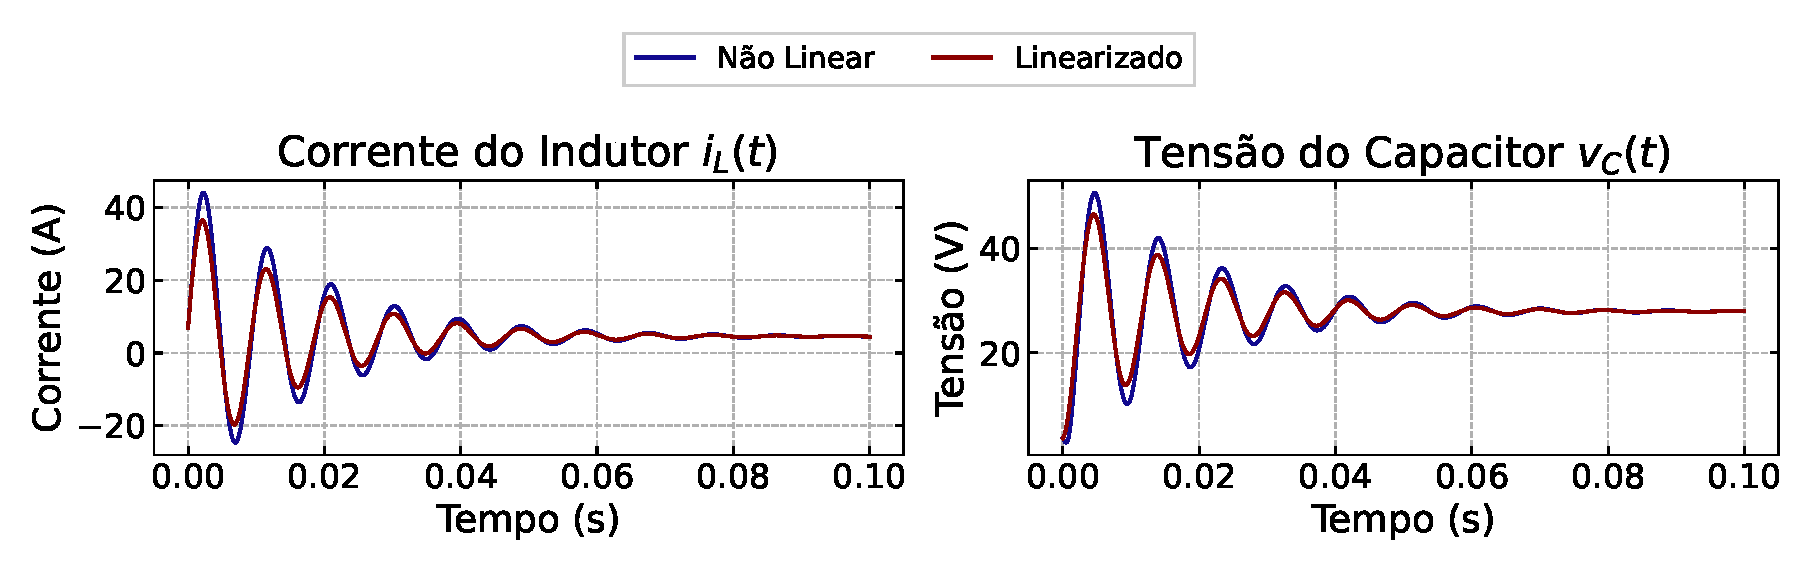
\includegraphics[width=1.\textwidth]{figuras/static-etm/buck/sim1/op1/result.eps}
    \caption{Estados do conversor.}
    \label{fig:buck_converter_constant_pcpl_static_etm_op1_duty_a}
  \end{subfigure}
  \\[6pt]
  \begin{subfigure}{1.\textwidth}
    \centering
    \includegraphics[width=1.\textwidth]{figuras/static-etm/buck/sim1/op1/duty-cycle.eps}
    \caption{Duty Cycle $d(t)$}
    \label{fig:buck_converter_constant_pcpl_static_etm_op1_duty_b}
  \end{subfigure}
  \\[6pt]
  \begin{subfigure}{1.\textwidth}
    \centering
    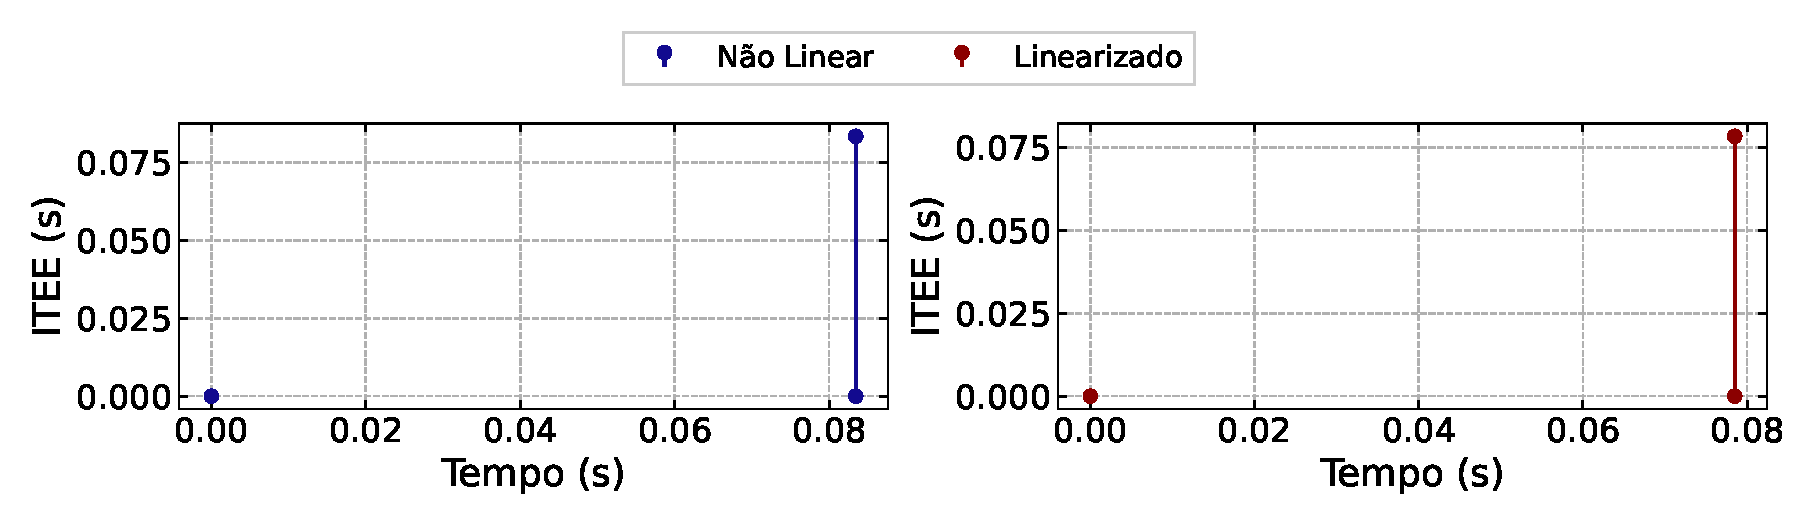
\includegraphics[width=1.\textwidth]{figuras/static-etm/buck/sim1/op1/inter-event-times.eps}
    \caption{Intervalo de tempo entre eventos.}
    \label{fig:buck_converter_constant_pcpl_static_etm_op1_duty_c}
  \end{subfigure}
  \caption{Entrada duty cycle $d(t)$ e os \acrshortpl{itee} do conversor Buck em torno do ponto $P_{\mathrm{o}, 1}$ sob sinal de pertubação $P_{\mathrm{cpl}}(t)$ constante e \acrshort{etm} estático.}
\end{figure}

Por outro lado, durante a simulação do conversor Buck em torno do ponto $P_{\mathrm{o}, 2}$, observou-se que o \acrshort{etm} desencadeou uma série de novos eventos, como mostrado na \autoref{fig:buck_converter_constant_pcpl_static_etm_op2_duty_b}. Esse padrão de comportamento era previsto devido à instabilidade associada ao ponto $P_{\mathrm{o}, 2}$. À medida que o sistema tende a se desviar gradualmente nesse ponto, o erro de transmissão aumenta, resultando na função de acionamento $\Gamma$ do \acrshort{etm} tornando-se negativa, o que permite o disparo de novos eventos de transmissão. Esse ciclo pode se repetir várias vezes ao longo do tempo, mesmo que o sistema, em malha fechada, eventualmente se estabilize. Portanto, é esperado que o \acrshort{etm} continue a realizar acionamentos mesmo após a estabilização do sistema.

\begin{figure}[H]
  \centering
  \captionsetup{justification=centering}
  \begin{subfigure}{1.\textwidth}
    \centering
    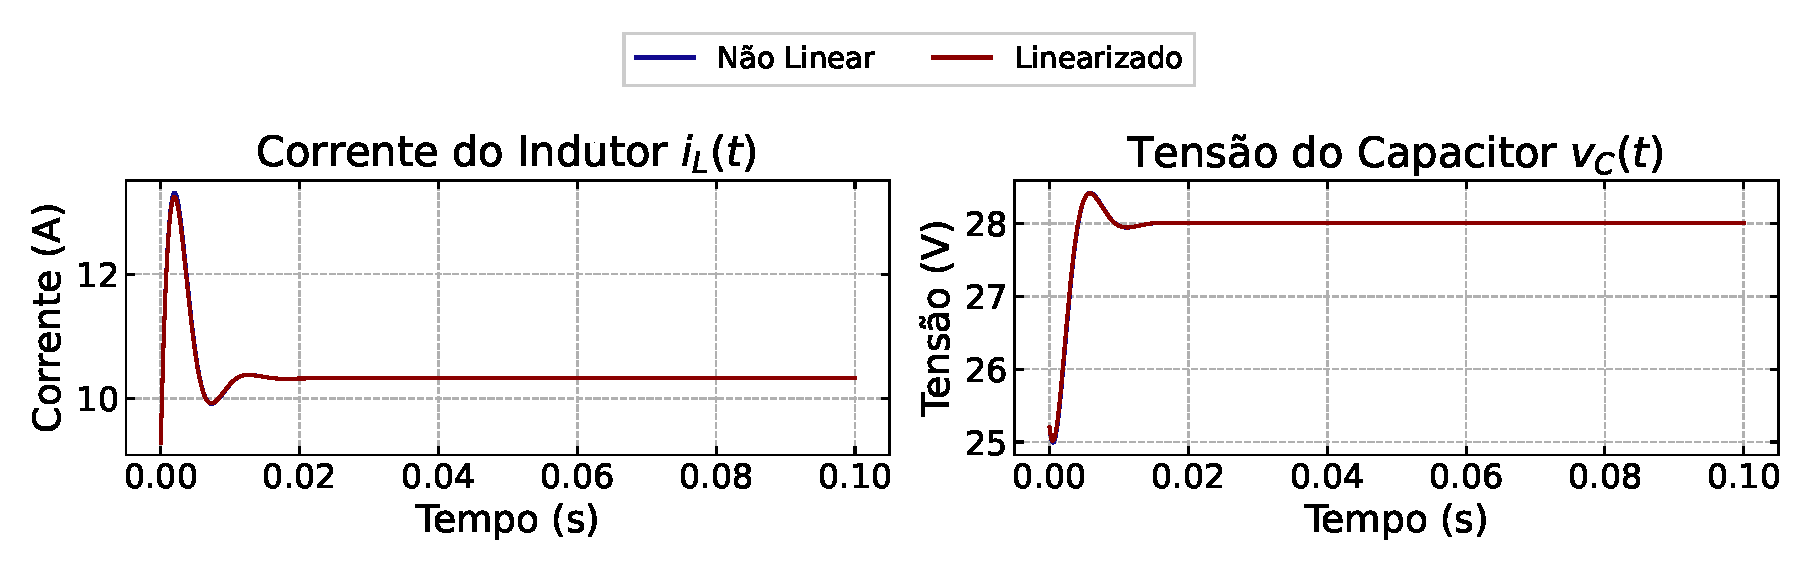
\includegraphics[width=1.\textwidth]{figuras/static-etm/buck/sim1/op2/result.eps}
    \caption{Estados do conversor.}
    \label{fig:buck_converter_constant_pcpl_static_etm_op2_duty_a}
  \end{subfigure}
  \\[6pt]
  \begin{subfigure}{1.\textwidth}
    \centering
    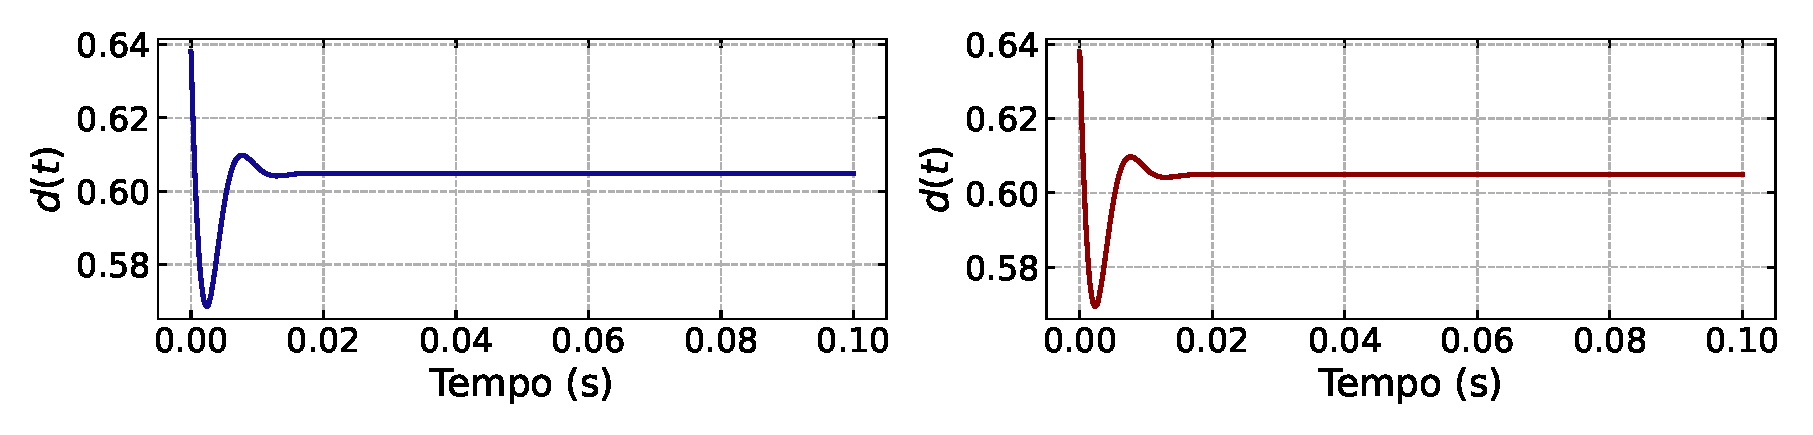
\includegraphics[width=1.\textwidth]{figuras/static-etm/buck/sim1/op2/duty-cycle.eps}
    \caption{Duty Cycle $d(t)$}
    \label{fig:buck_converter_constant_pcpl_static_etm_op2_duty_b}
  \end{subfigure}
  \\[6pt]
  \begin{subfigure}{1.\textwidth}
    \centering
    \includegraphics[width=1.\textwidth]{figuras/static-etm/buck/sim1/op2/inter-event-times.eps}
    \caption{Intervalo de tempo entre eventos.}
    \label{fig:buck_converter_constant_pcpl_static_etm_op2_duty_c}
  \end{subfigure}
  \caption{Entrada duty cycle $d(t)$ e os \acrshortpl{itee} do conversor Buck em torno do ponto $P_{\mathrm{o}, 2}$ sob sinal de pertubação $P_{\mathrm{cpl}}(t)$ constante e \acrshort{etm} estático.}
\end{figure}


\subsubsection{Sinal de Pertubação Variável}

\begin{figure}[H]
  \centering
  \captionsetup{justification=centering}
  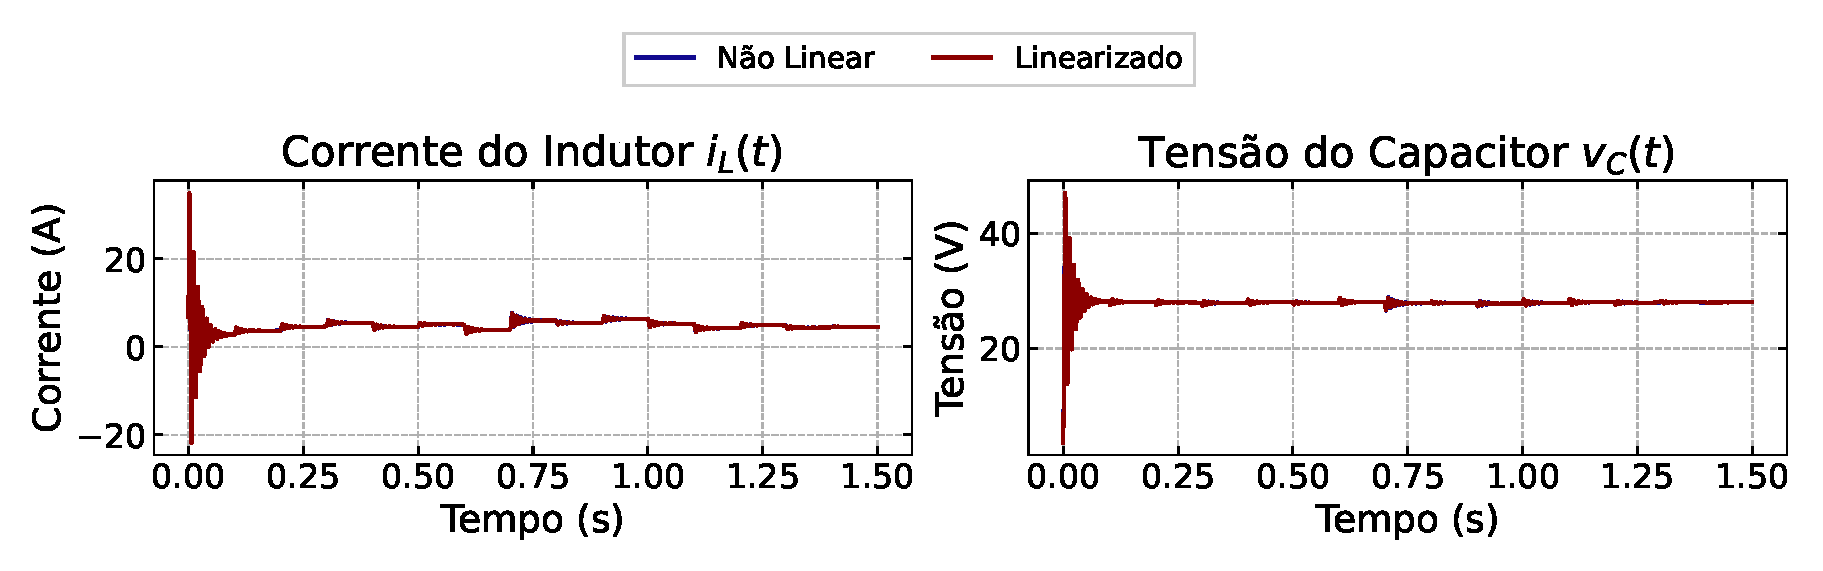
\includegraphics[width=1.\textwidth]{figuras/static-etm/buck/sim2/op1/result.eps}
  \caption{Estados do conversor Buck em torno do ponto de operação $P_{\mathrm{o}, 1}$ sob sinal de pertubação $P_{\mathrm{cpl}}(t)$ variável e \acrshort{etm} estático.}
  % \label{fig:simulation_2_boost_op2}
\end{figure}

\begin{figure}[H]
  \centering
  \captionsetup{justification=centering}
  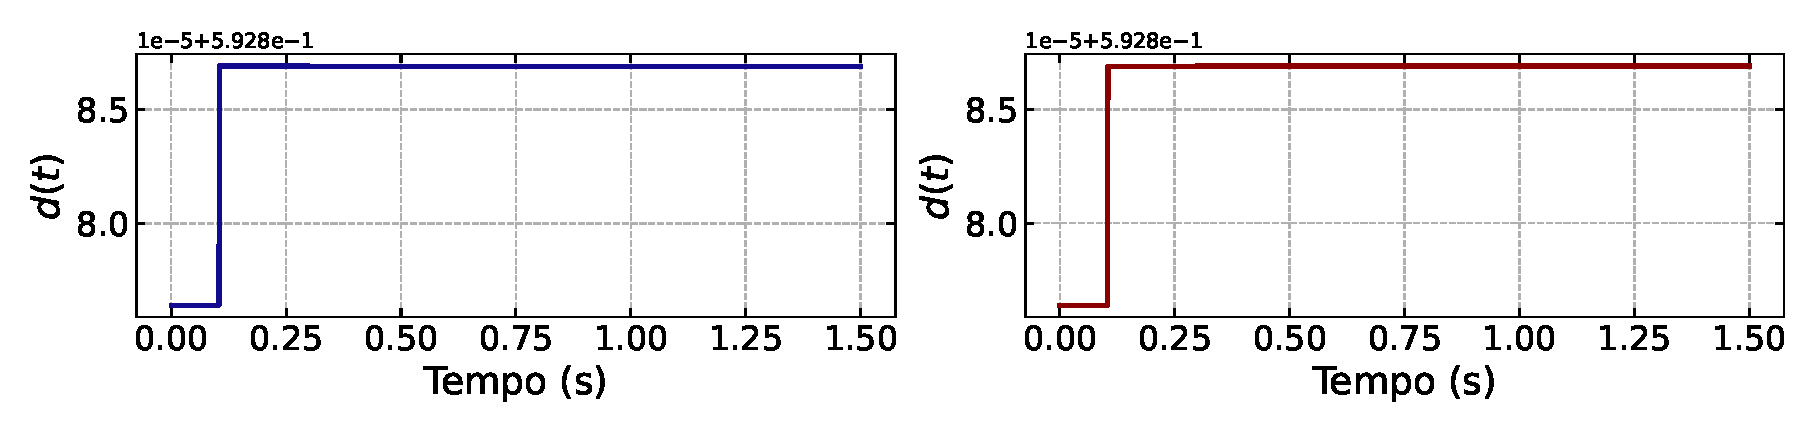
\includegraphics[width=1.\textwidth]{figuras/static-etm/buck/sim2/op1/duty-cycle.eps}
  \caption{Entrada duty cycle $d(t)$ do conversor Buck em torno do ponto de operação $P_{\mathrm{o}, 1}$ sob sinal de pertubação $P_{\mathrm{cpl}}(t)$ variável e \acrshort{etm} estático.}
  % \label{fig:simulation_2_boost_op2}
\end{figure}

\begin{figure}[H]
  \centering
  \captionsetup{justification=centering}
  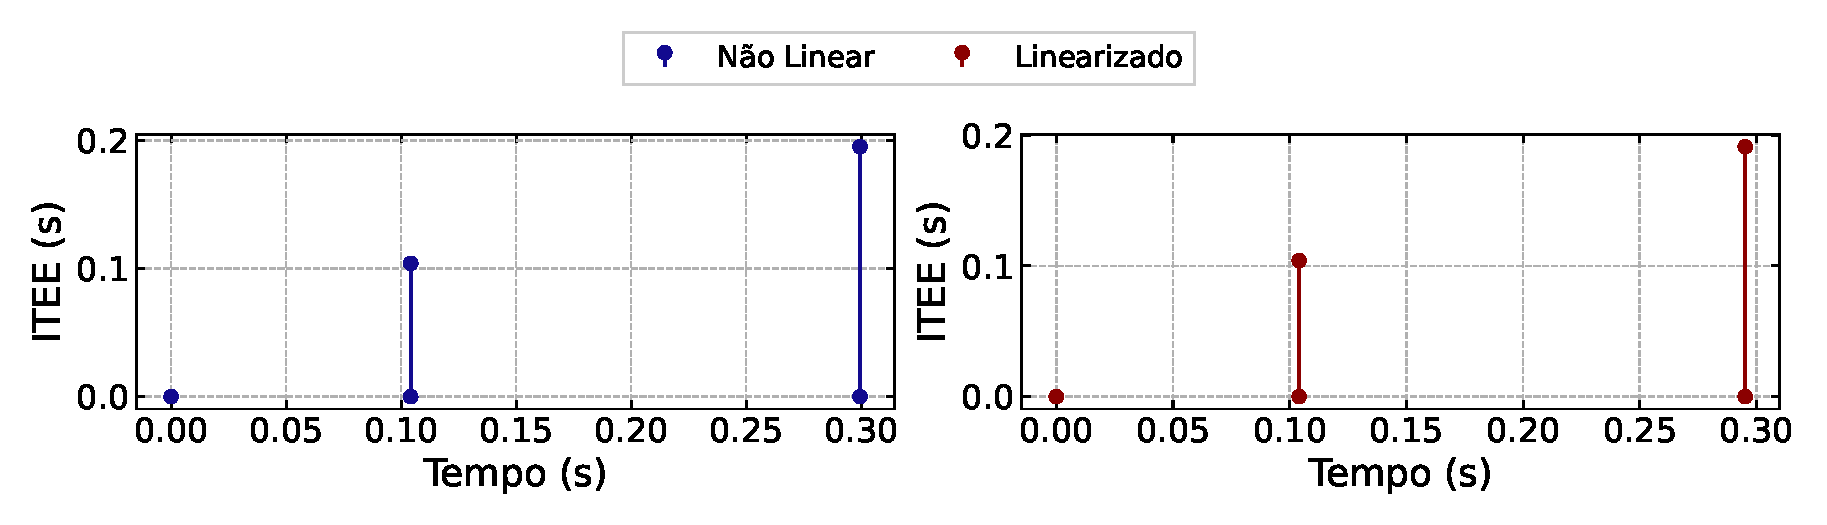
\includegraphics[width=1.\textwidth]{figuras/static-etm/buck/sim2/op1/inter-event-times.eps}
  \caption{Tempo entre evento do conversor Buck em torno do ponto de operação $P_{\mathrm{o}, 1}$ sob sinal de pertubação $P_{\mathrm{cpl}}(t)$ variável e \acrshort{etm} estático.}
  % \label{fig:simulation_2_boost_op2}
\end{figure}

% Instável

\begin{figure}[H]
  \centering
  \captionsetup{justification=centering}
  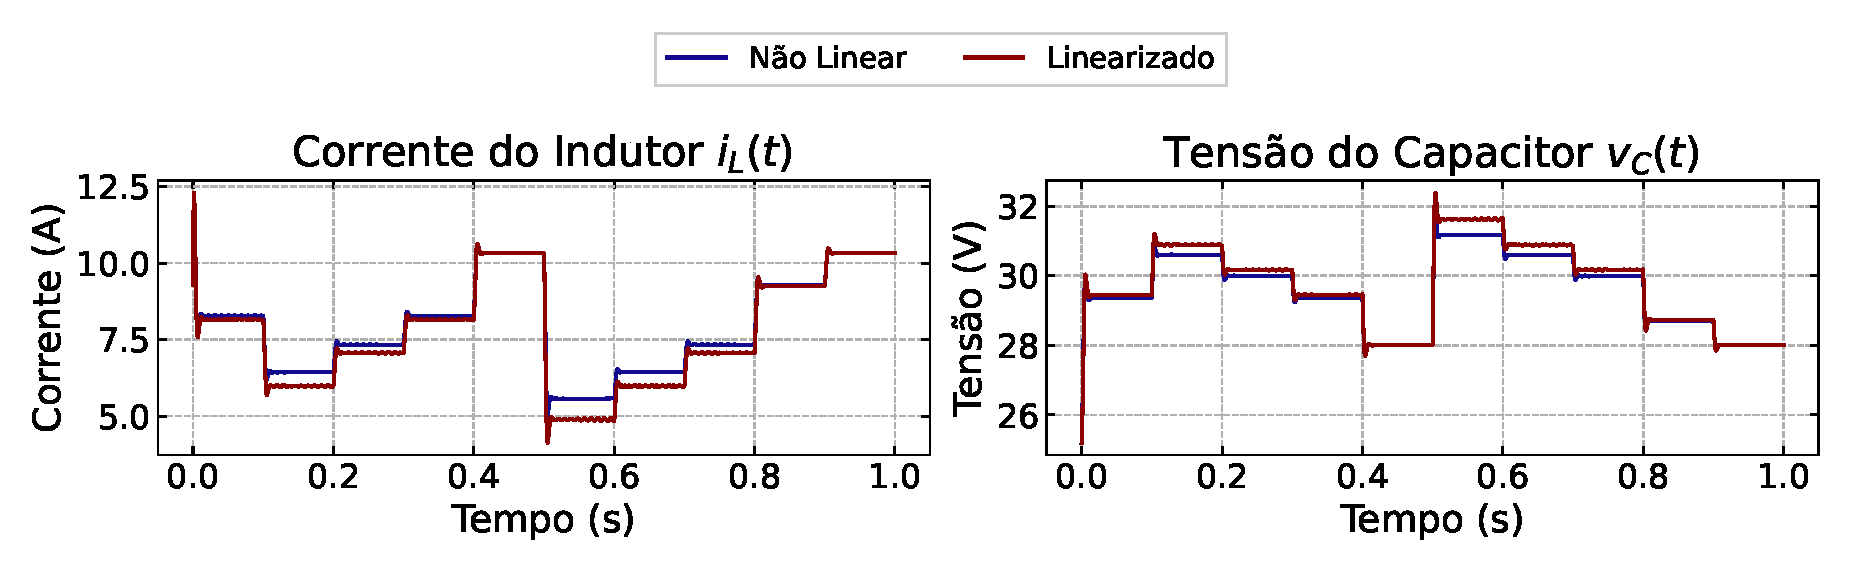
\includegraphics[width=1.\textwidth]{figuras/static-etm/buck/sim2/op2/result.eps}
  \caption{Estados do conversor Buck em torno do ponto de operação $P_{\mathrm{o}, 2}$ sob sinal de pertubação $P_{\mathrm{cpl}}(t)$ variável e \acrshort{etm} estático.}
  % \label{fig:simulation_2_boost_op2}
\end{figure}

\begin{figure}[H]
  \centering
  \captionsetup{justification=centering}
  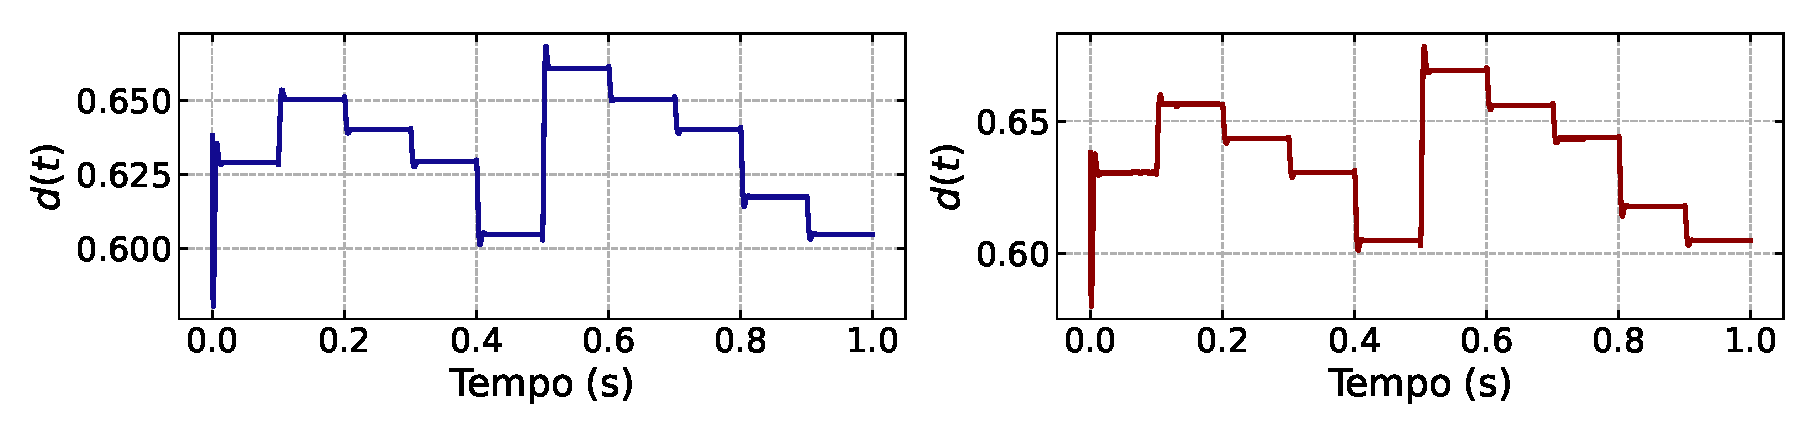
\includegraphics[width=1.\textwidth]{figuras/static-etm/buck/sim2/op2/duty-cycle.eps}
  \caption{Entrada duty cycle $d(t)$ do conversor Buck em torno do ponto de operação $P_{\mathrm{o}, 2}$ sob sinal de pertubação $P_{\mathrm{cpl}}(t)$ variável e \acrshort{etm} estático.}
  % \label{fig:simulation_2_boost_op2}
\end{figure}

\begin{figure}[H]
  \centering
  \captionsetup{justification=centering}
  \includegraphics[width=1.\textwidth]{figuras/static-etm/buck/sim2/op2/inter-event-times.eps}
  \caption{Tempo entre evento do conversor Buck em torno do ponto de operação $P_{\mathrm{o}, 2}$ sob sinal de pertubação $P_{\mathrm{cpl}}(t)$ variável e \acrshort{etm} estático.}
  % \label{fig:simulation_2_boost_op2}
\end{figure}

\subsection{Conversor Boost}
\subsubsection{Sinal de Pertubação Constante}

\begin{figure}[H]
  \centering
  \captionsetup{justification=centering}
  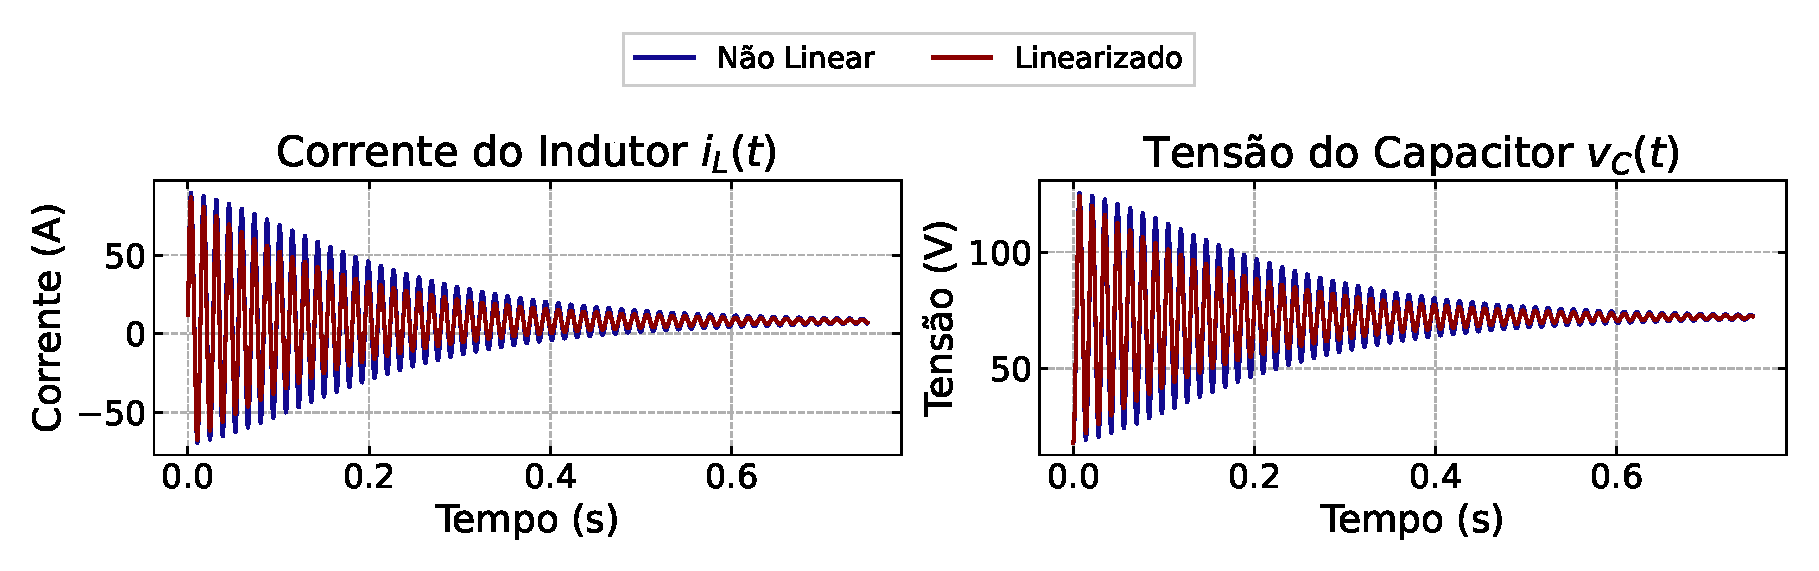
\includegraphics[width=1.\textwidth]{figuras/static-etm/boost/sim1/op1/result.eps}
  \caption{Estados do conversor Boost em torno do ponto de operação $P_{\mathrm{o}, 3}$ sob sinal de pertubação $P_{\mathrm{cpl}}(t)$ constante e \acrshort{etm} estático.}
  % \label{fig:simulation_2_boost_op2}
\end{figure}

\begin{figure}[H]
  \centering
  \captionsetup{justification=centering}
  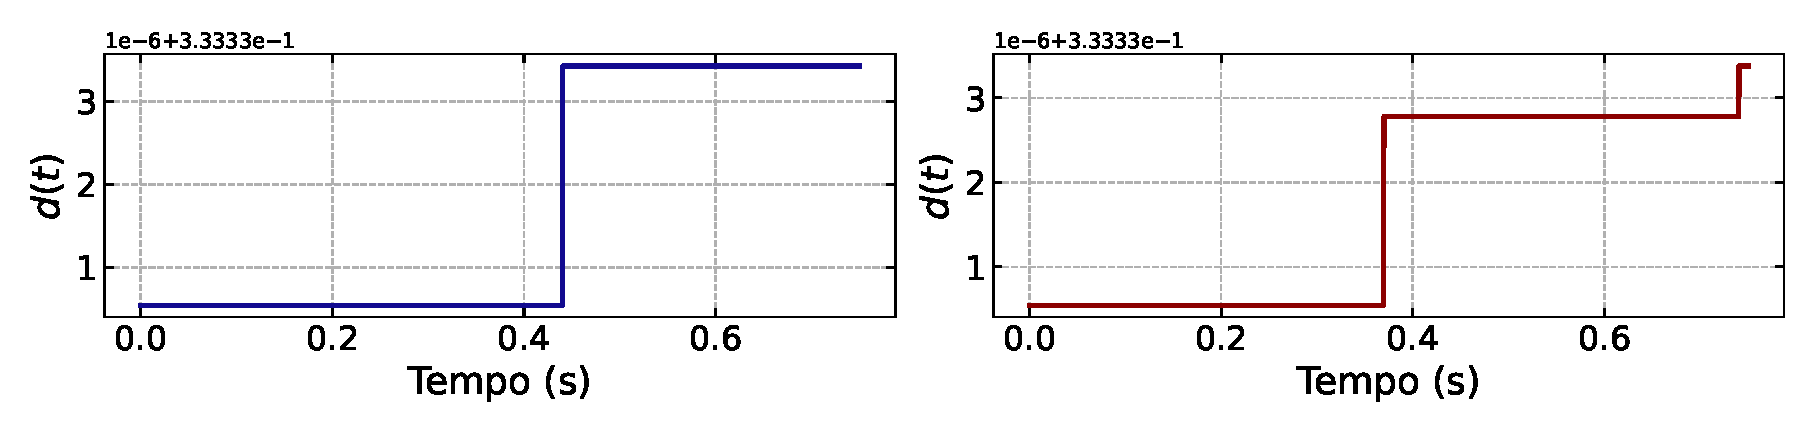
\includegraphics[width=1.\textwidth]{figuras/static-etm/boost/sim1/op1/duty-cycle.eps}
  \caption{Entrada duty cycle $d(t)$ do conversor Boost em torno do ponto de operação $P_{\mathrm{o}, 3}$ sob sinal de pertubação $P_{\mathrm{cpl}}(t)$ constante e \acrshort{etm} estático.}
  % \label{fig:simulation_2_boost_op2}
\end{figure}

\begin{figure}[H]
  \centering
  \captionsetup{justification=centering}
  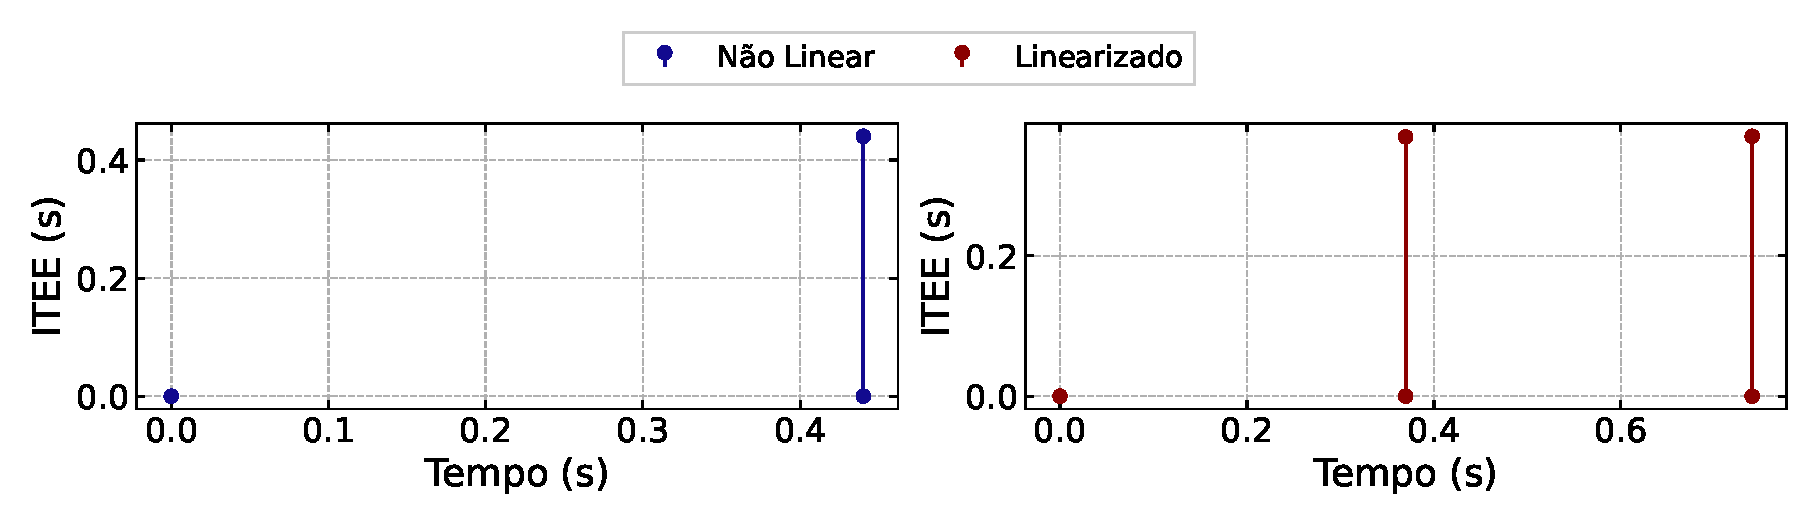
\includegraphics[width=1.\textwidth]{figuras/static-etm/boost/sim1/op1/inter-event-times.eps}
  \caption{Tempo entre evento do conversor Boost em torno do ponto de operação $P_{\mathrm{o}, 3}$ sob sinal de pertubação $P_{\mathrm{cpl}}(t)$ constante e \acrshort{etm} estático.}
  % \label{fig:simulation_2_boost_op2}
\end{figure}

\begin{figure}[H]
  \centering
  \captionsetup{justification=centering}
  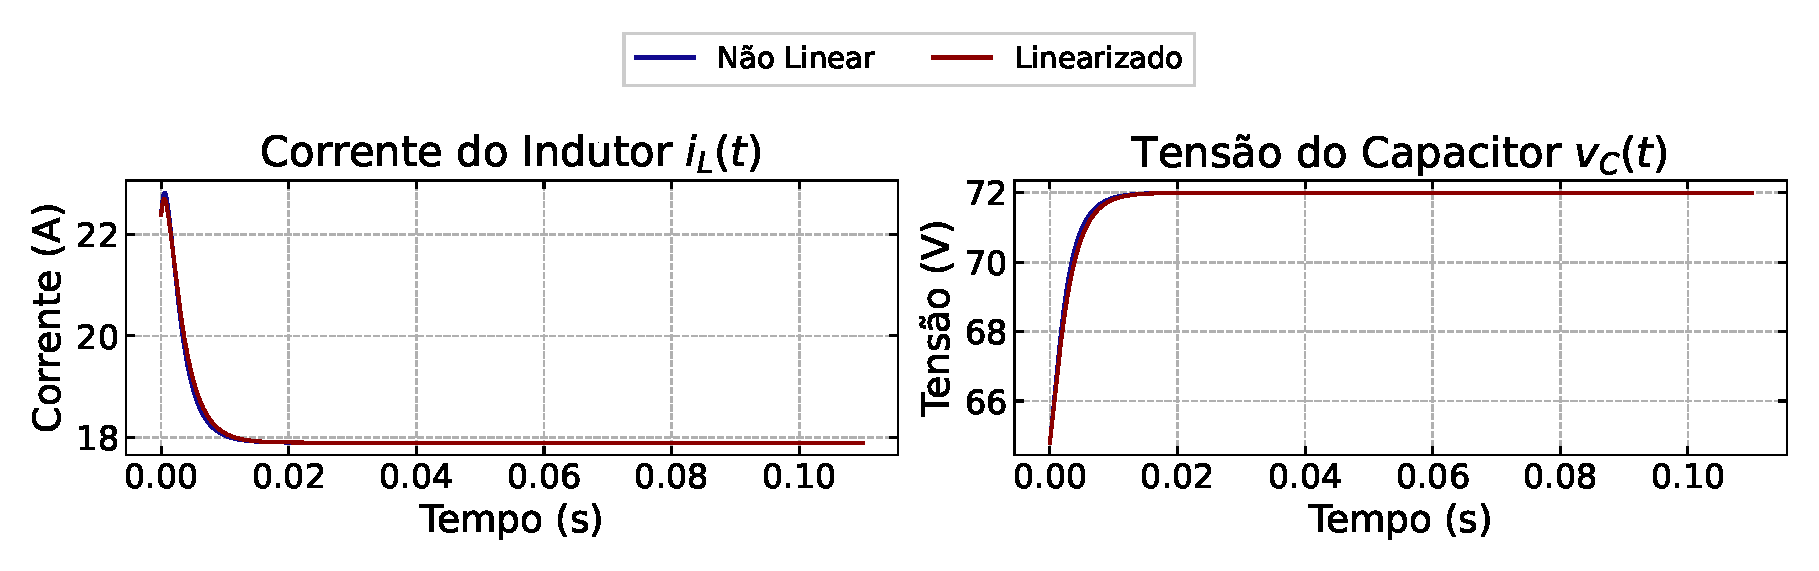
\includegraphics[width=1.\textwidth]{figuras/static-etm/boost/sim1/op2/result.eps}
  \caption{Estados do conversor Boost em torno do ponto de operação $P_{\mathrm{o}, 4}$ sob sinal de pertubação $P_{\mathrm{cpl}}(t)$ constante e \acrshort{etm} estático.}
  % \label{fig:simulation_2_boost_op2}
\end{figure}

\begin{figure}[H]
  \centering
  \captionsetup{justification=centering}
  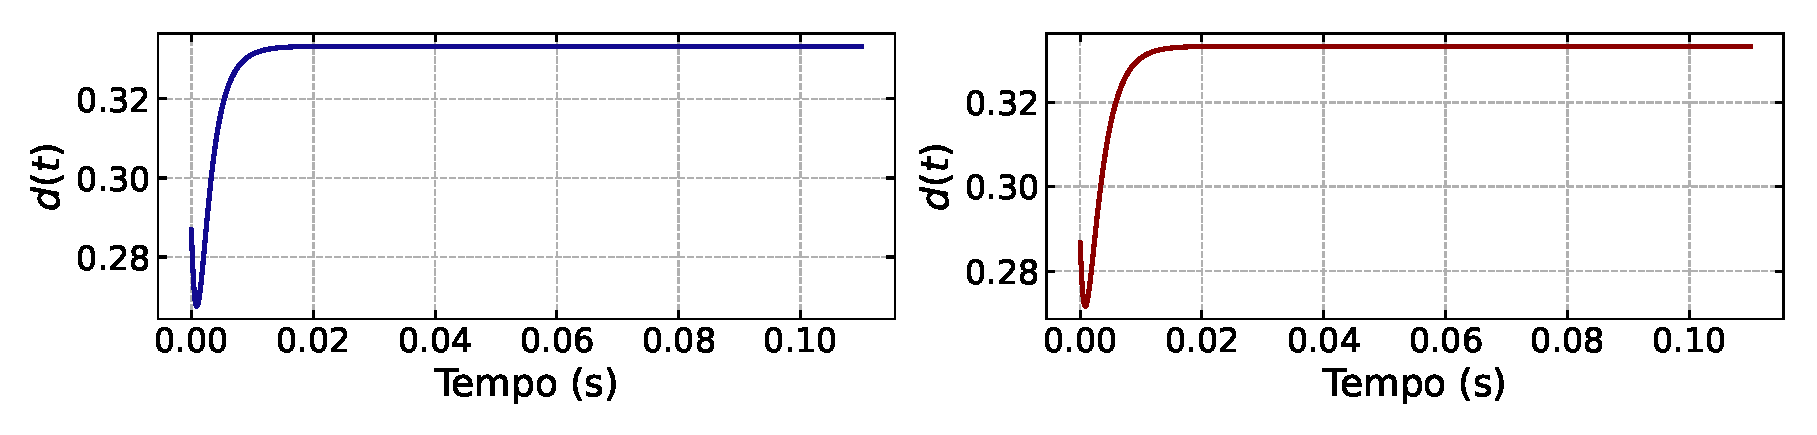
\includegraphics[width=1.\textwidth]{figuras/static-etm/boost/sim1/op2/duty-cycle.eps}
  \caption{Entrada duty cycle $d(t)$ do conversor Boost em torno do ponto de operação $P_{\mathrm{o}, 4}$ sob sinal de pertubação $P_{\mathrm{cpl}}(t)$ constante e \acrshort{etm} estático.}
  % \label{fig:simulation_2_boost_op2}
\end{figure}

\begin{figure}[H]
  \centering
  \captionsetup{justification=centering}
  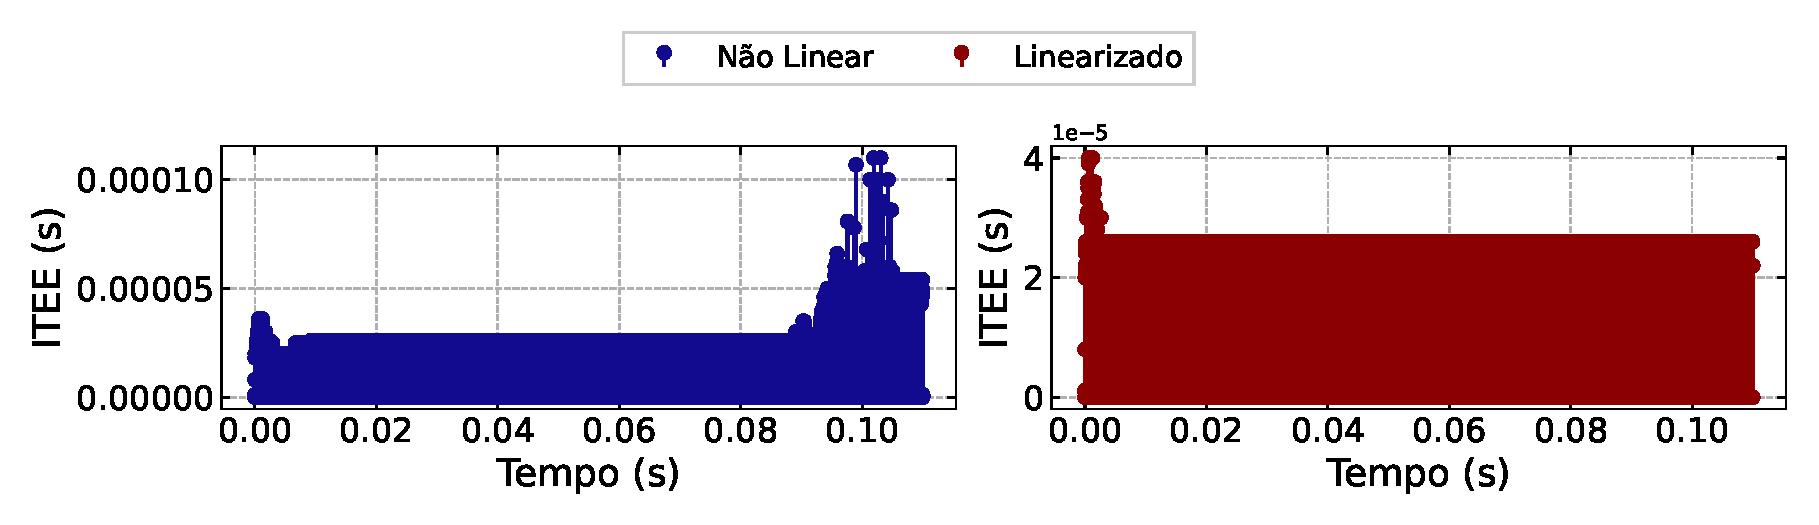
\includegraphics[width=1.\textwidth]{figuras/static-etm/boost/sim1/op2/inter-event-times.eps}
  \caption{Tempo entre evento do conversor Boost em torno do ponto de operação $P_{\mathrm{o}, 4}$ sob sinal de pertubação $P_{\mathrm{cpl}}(t)$ constante e \acrshort{etm} estático.}
  % \label{fig:simulation_2_boost_op2}
\end{figure}

\subsubsection{Sinal de Pertubação Variável}

\begin{figure}[H]
  \centering
  \captionsetup{justification=centering}
  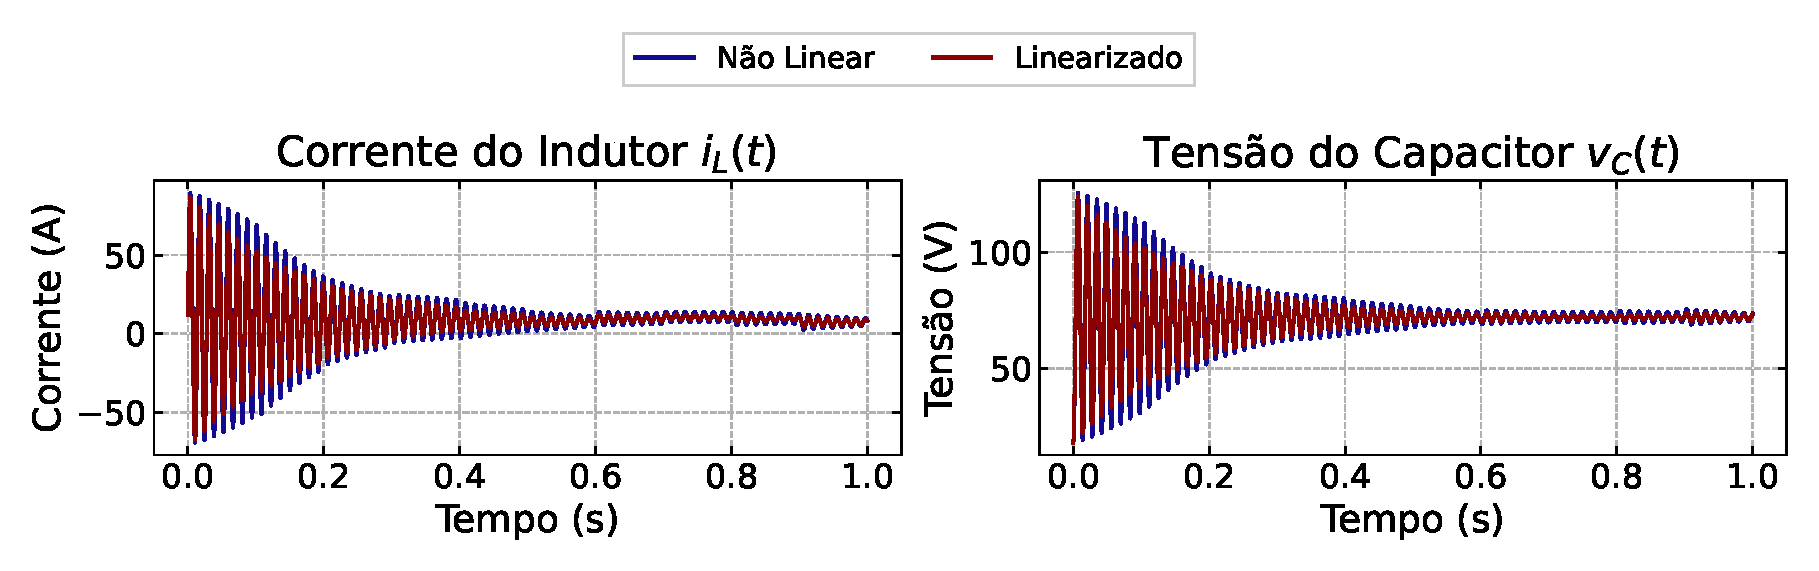
\includegraphics[width=1.\textwidth]{figuras/static-etm/boost/sim2/op1/result.eps}
  \caption{Estados do conversor Boost em torno do ponto de operação $P_{\mathrm{o}, 3}$ sob sinal de pertubação $P_{\mathrm{cpl}}(t)$ variável e \acrshort{etm} estático.}
  % \label{fig:simulation_2_boost_op2}
\end{figure}

\begin{figure}[H]
  \centering
  \captionsetup{justification=centering}
  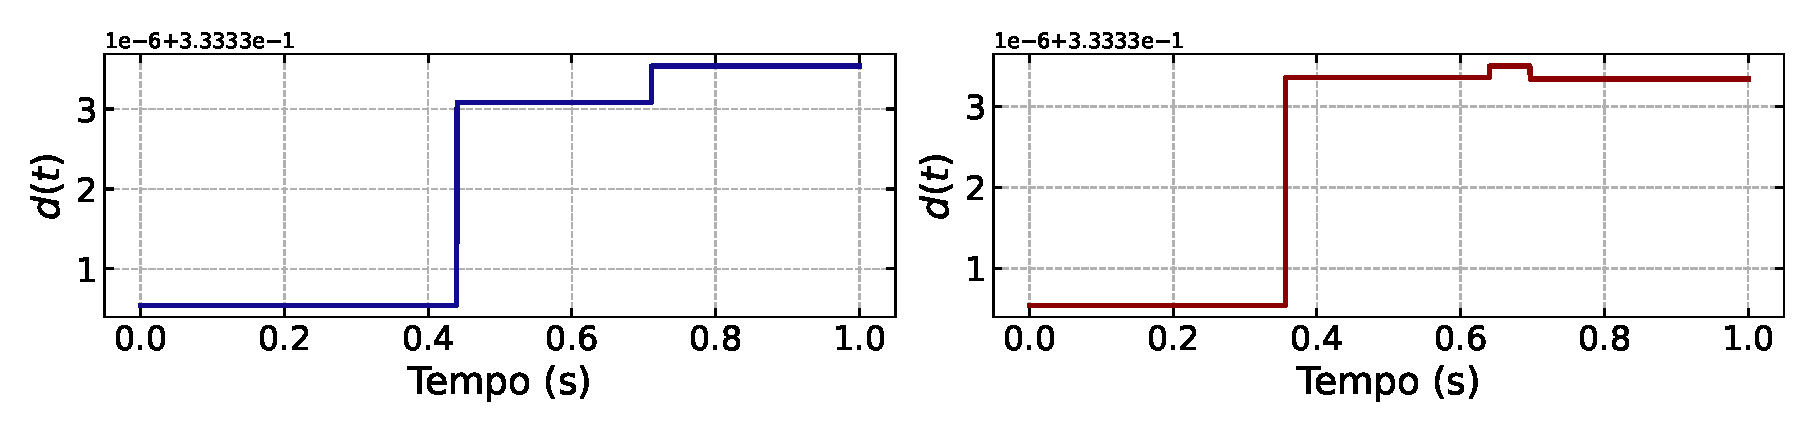
\includegraphics[width=1.\textwidth]{figuras/static-etm/boost/sim2/op1/duty-cycle.eps}
  \caption{Entrada duty cycle $d(t)$ do conversor Boost em torno do ponto de operação $P_{\mathrm{o}, 3}$ sob sinal de pertubação $P_{\mathrm{cpl}}(t)$ variável e \acrshort{etm} estático.}
  % \label{fig:simulation_2_boost_op2}
\end{figure}

\begin{figure}[H]
  \centering
  \captionsetup{justification=centering}
  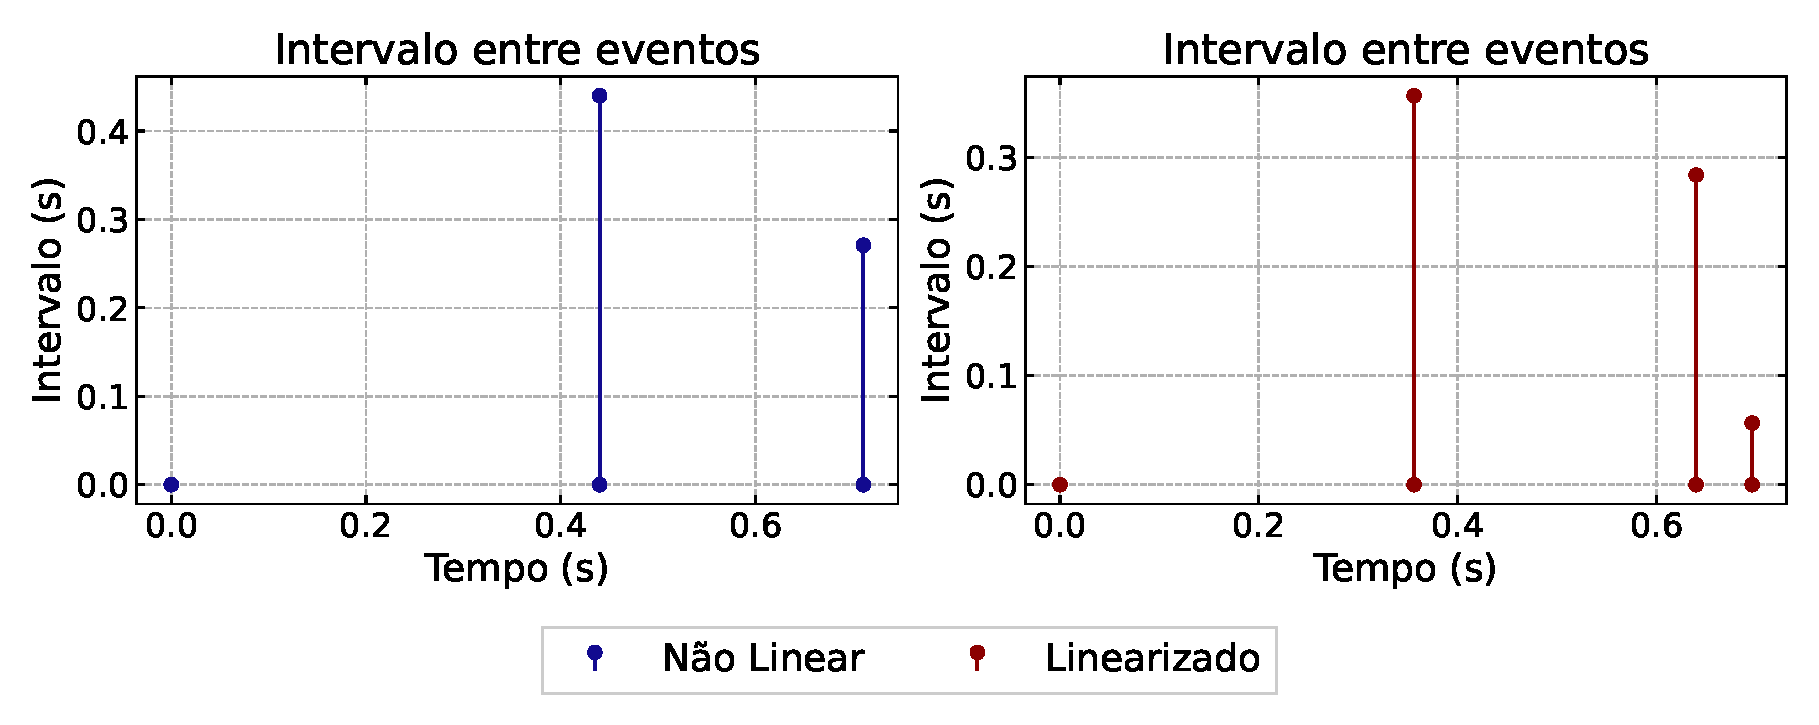
\includegraphics[width=1.\textwidth]{figuras/static-etm/boost/sim2/op1/inter-event-times.eps}
  \caption{Tempo entre evento do conversor Boost em torno do ponto de operação $P_{\mathrm{o}, 3}$ sob sinal de pertubação $P_{\mathrm{cpl}}(t)$ variável e \acrshort{etm} estático.}
  % \label{fig:simulation_2_boost_op2}
\end{figure}

\begin{figure}[H]
  \centering
  \captionsetup{justification=centering}
  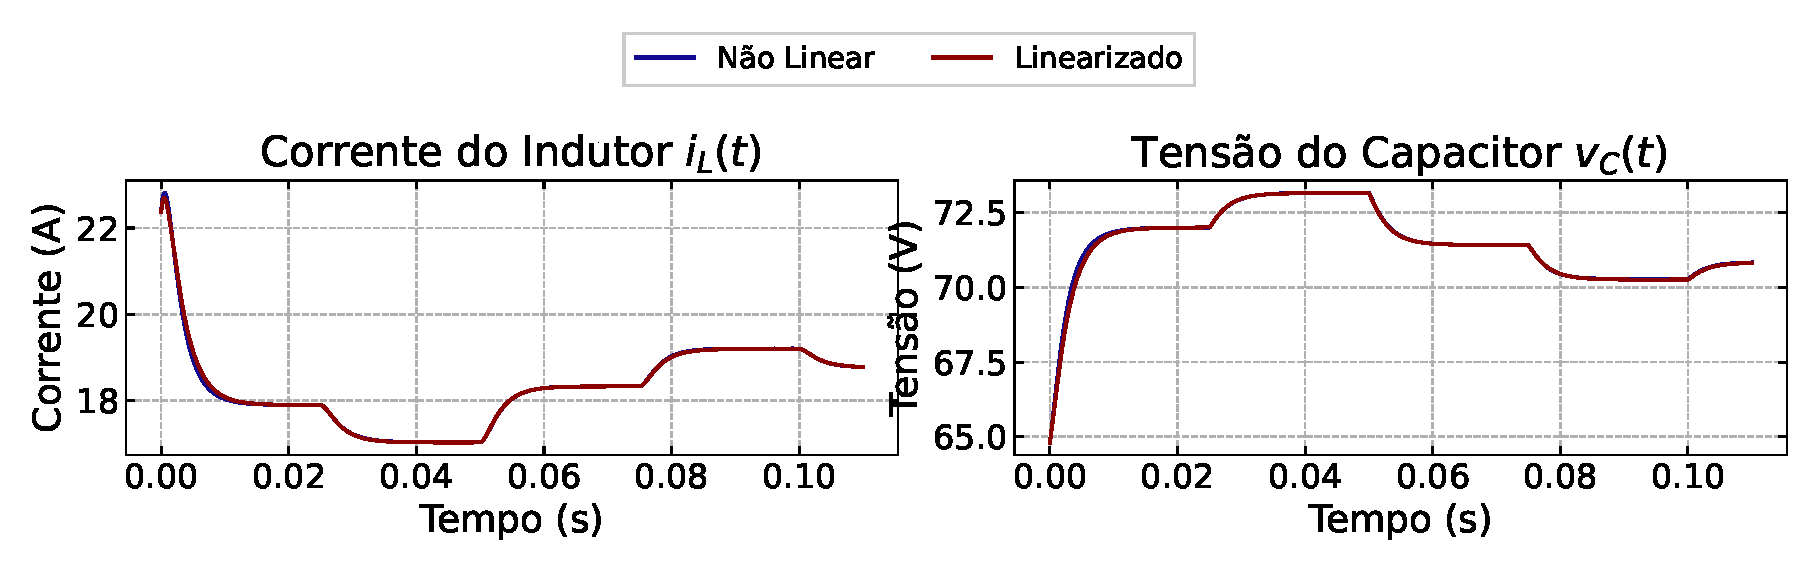
\includegraphics[width=1.\textwidth]{figuras/static-etm/boost/sim2/op2/result.eps}
  \caption{Estados do conversor Boost em torno do ponto de operação $P_{\mathrm{o}, 4}$ sob sinal de pertubação $P_{\mathrm{cpl}}(t)$ variável e \acrshort{etm} estático.}
  % \label{fig:simulation_2_boost_op2}
\end{figure}

\begin{figure}[H]
  \centering
  \captionsetup{justification=centering}
  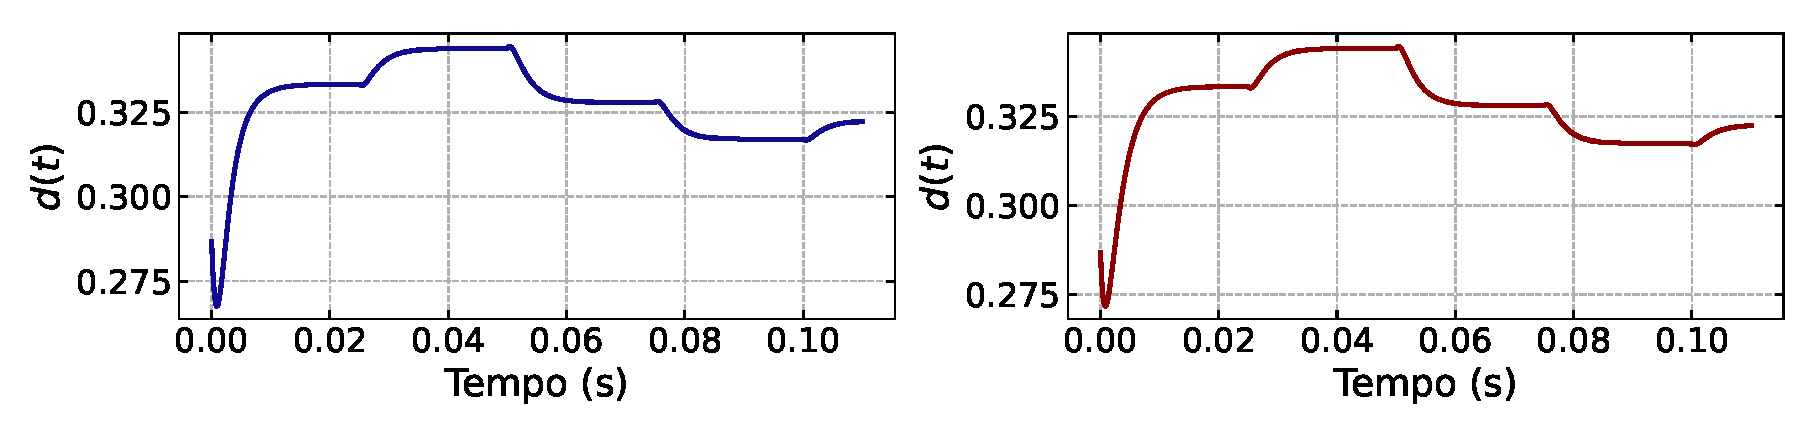
\includegraphics[width=1.\textwidth]{figuras/static-etm/boost/sim2/op2/duty-cycle.eps}
  \caption{Entrada duty cycle $d(t)$ do conversor Boost em torno do ponto de operação $P_{\mathrm{o}, 4}$ sob sinal de pertubação $P_{\mathrm{cpl}}(t)$ variável e \acrshort{etm} estático.}
  % \label{fig:simulation_2_boost_op2}
\end{figure}

\begin{figure}[H]
  \centering
  \captionsetup{justification=centering}
  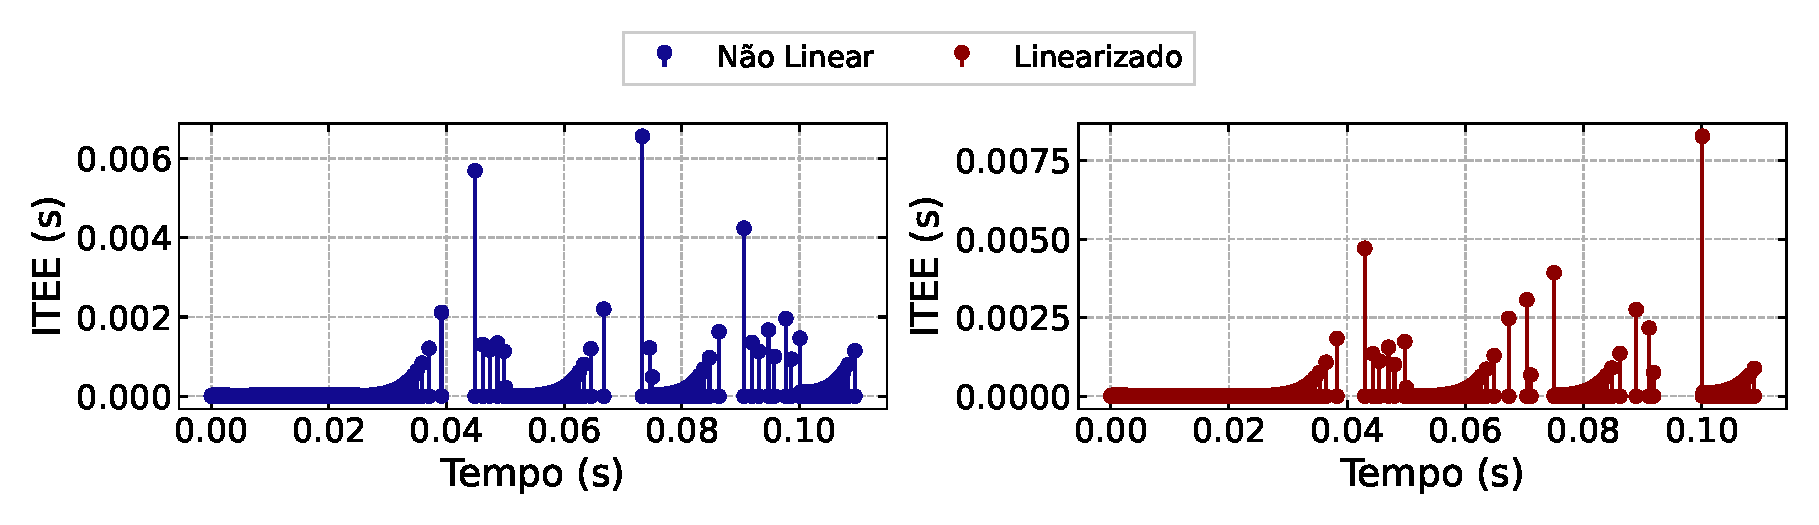
\includegraphics[width=1.\textwidth]{figuras/static-etm/boost/sim2/op2/inter-event-times.eps}
  \caption{Tempo entre evento do conversor Boost em torno do ponto de operação $P_{\mathrm{o}, 4}$ sob sinal de pertubação $P_{\mathrm{cpl}}(t)$ variável e \acrshort{etm} estático.}
  % \label{fig:simulation_2_boost_op2}
\end{figure}

\section{Conversores em Malha Fechada sob \acrshort{etm} Dinâmico}

\subsection{Conversor Buck}

\subsubsection{Sinal de Pertubação Constante}

% Estável

\begin{figure}[H]
  \centering
  \captionsetup{justification=centering}
  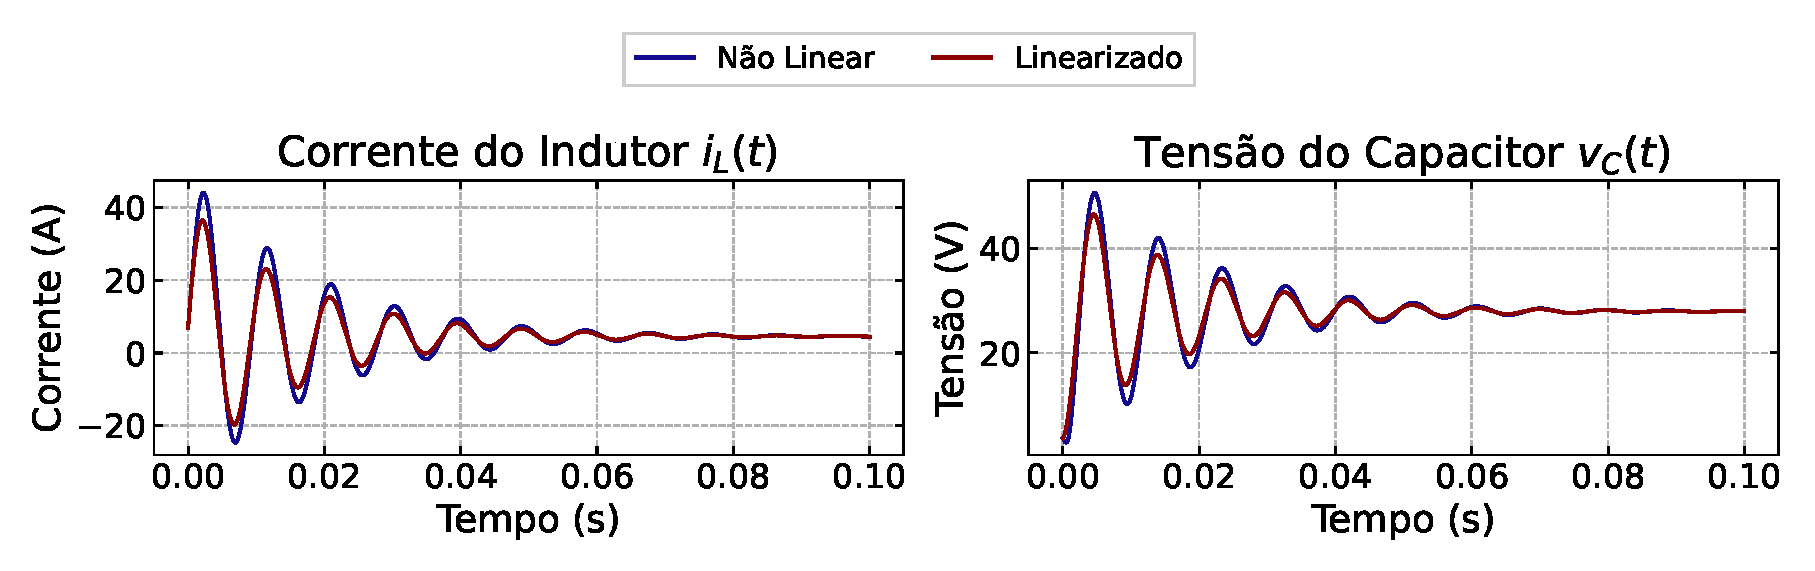
\includegraphics[width=1.\textwidth]{figuras/dynamic-etm/buck/sim1/op1/result.eps}
  \caption{Estados do conversor Buck em torno do ponto de operação $P_{\mathrm{o}, 1}$ sob sinal de pertubação $P_{\mathrm{cpl}}(t)$ constante e \acrshort{etm} estático.}
  % \label{fig:simulation_2_boost_op2}
\end{figure}

\begin{figure}[H]
  \centering
  \captionsetup{justification=centering}
  \includegraphics[width=1.\textwidth]{figuras/dynamic-etm/buck/sim1/op1/duty-cycle.eps}
  \caption{Entrada duty cycle $d(t)$ do conversor Buck em torno do ponto de operação $P_{\mathrm{o}, 1}$ sob sinal de pertubação $P_{\mathrm{cpl}}(t)$ constante e \acrshort{etm} estático.}
  % \label{fig:simulation_2_boost_op2}
\end{figure}

\begin{figure}[H]
  \centering
  \captionsetup{justification=centering}
  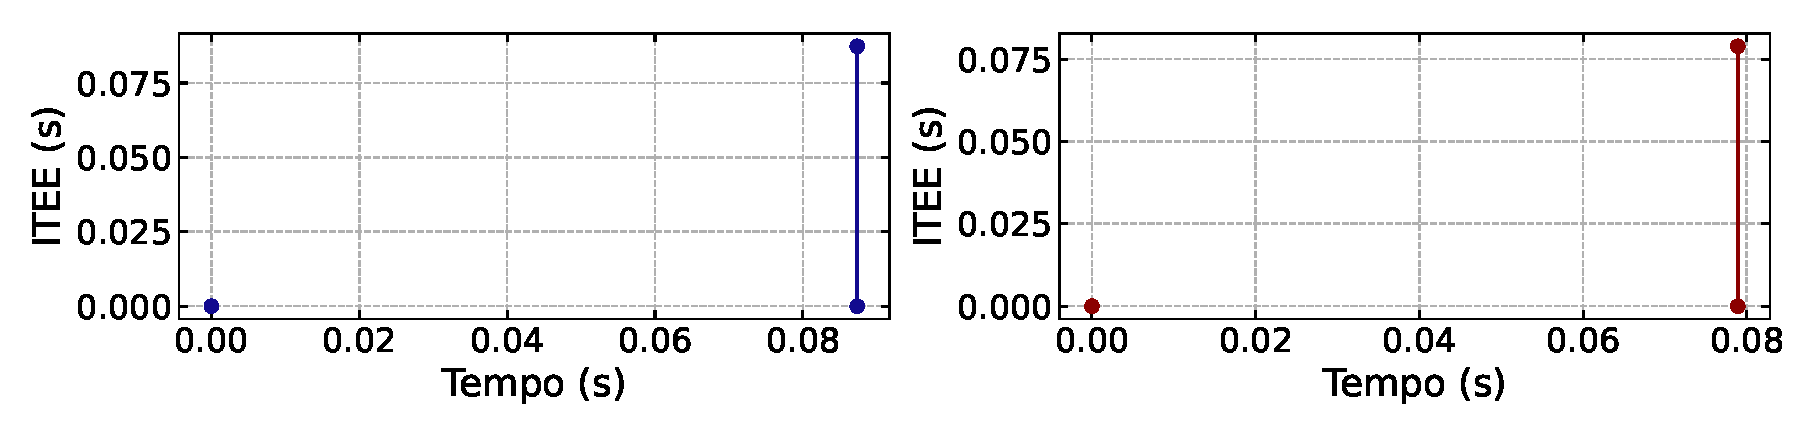
\includegraphics[width=1.\textwidth]{figuras/dynamic-etm/buck/sim1/op1/inter-event-times.eps}
  \caption{Tempo entre evento do conversor Buck em torno do ponto de operação $P_{\mathrm{o}, 1}$ sob sinal de pertubação $P_{\mathrm{cpl}}(t)$ constante e \acrshort{etm} estático.}
  % \label{fig:simulation_2_boost_op2}
\end{figure}

\begin{figure}[H]
  \centering
  \captionsetup{justification=centering}
  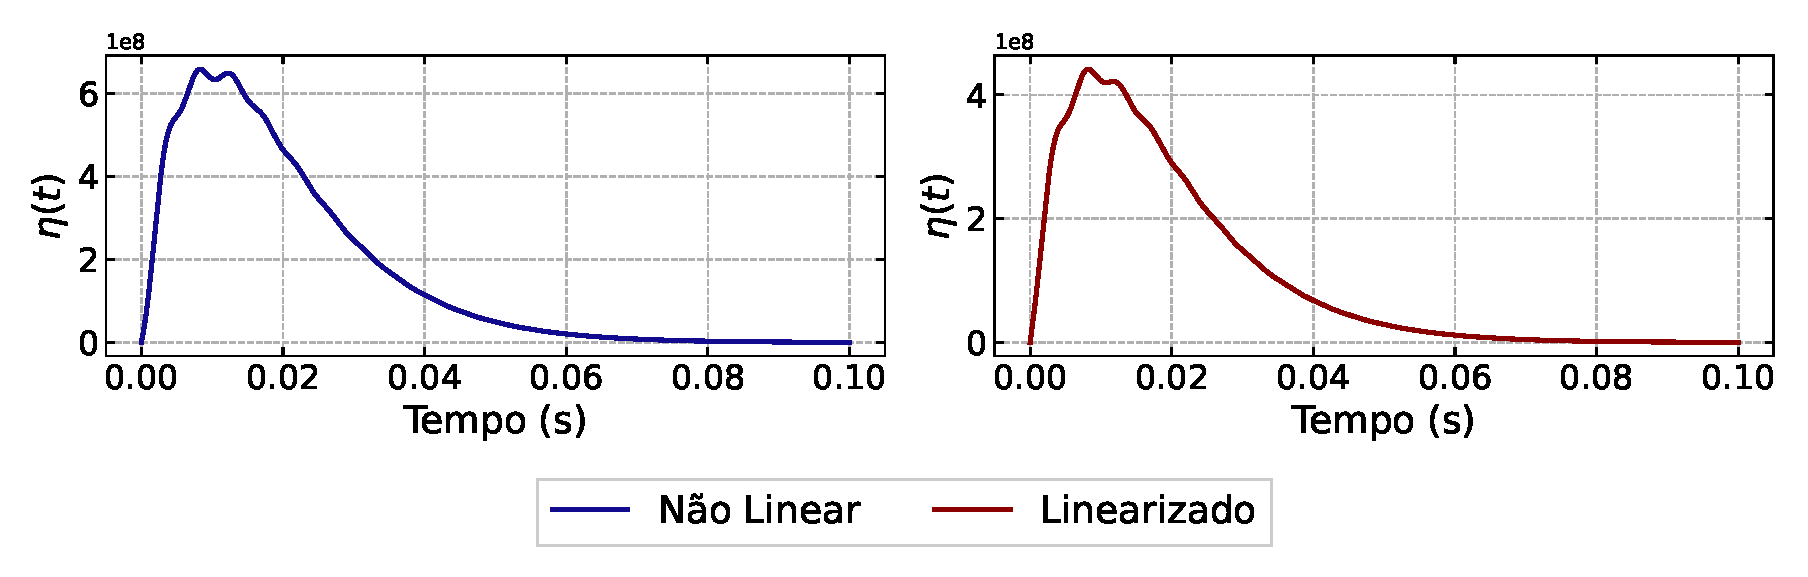
\includegraphics[width=1.\textwidth]{figuras/dynamic-etm/buck/sim1/op1/eta.eps}
  \caption{Variável dinâmica $\eta(t)$ do \acrshort{etm} dinâmico na simulação do conversor Buck em torno do ponto de operação $P_{\mathrm{o}, 1}$ sob sinal de pertubação $P_{\mathrm{cpl}}(t)$ constante.}
  % \label{fig:simulation_2_boost_op2}
\end{figure}

% % Instável

\begin{figure}[H]
  \centering
  \captionsetup{justification=centering}
  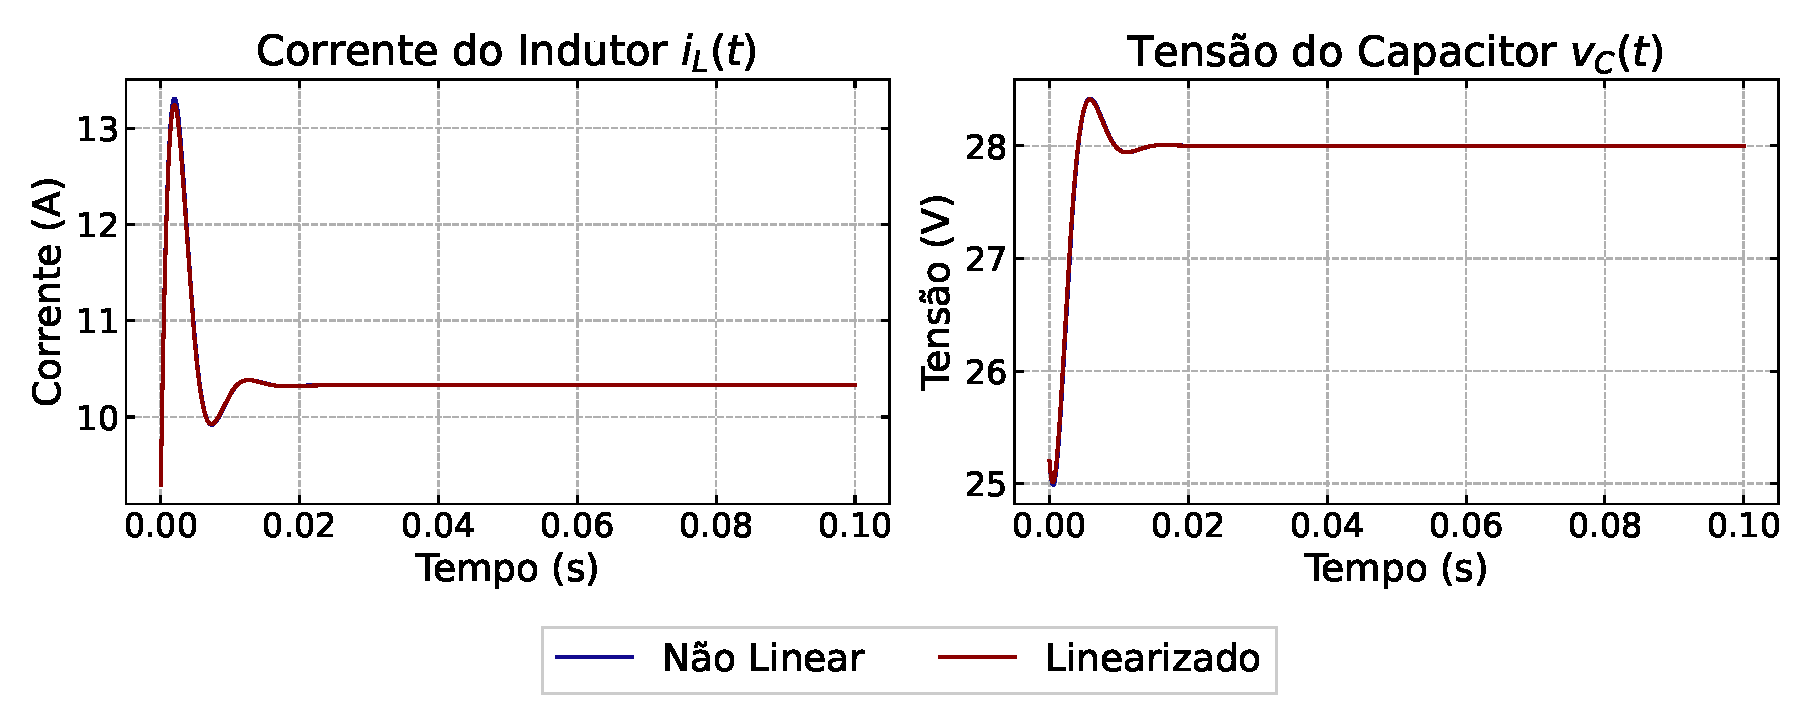
\includegraphics[width=1.\textwidth]{figuras/dynamic-etm/buck/sim1/op2/result.eps}
  \caption{Estados do conversor Buck em torno do ponto de operação $P_{\mathrm{o}, 2}$ sob sinal de pertubação $P_{\mathrm{cpl}}(t)$ constante e \acrshort{etm} estático.}
  % \label{fig:simulation_2_boost_op2}
\end{figure}

\begin{figure}[H]
  \centering
  \captionsetup{justification=centering}
  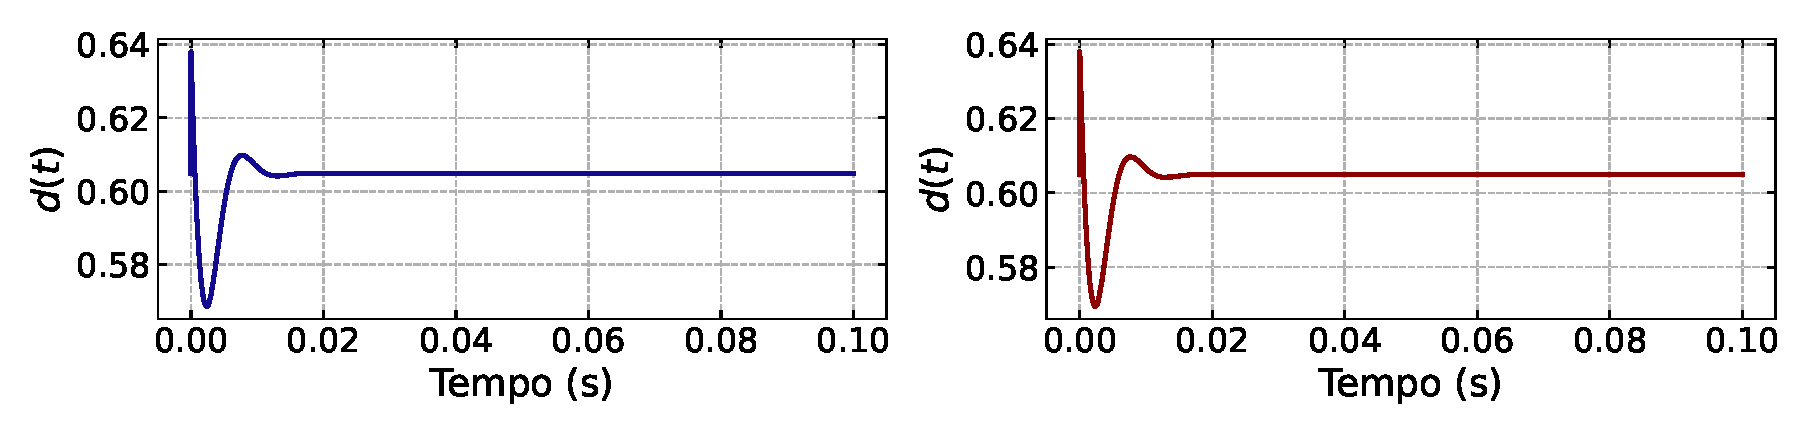
\includegraphics[width=1.\textwidth]{figuras/dynamic-etm/buck/sim1/op2/duty-cycle.eps}
  \caption{Entrada duty cycle $d(t)$ do conversor Buck em torno do ponto de operação $P_{\mathrm{o}, 2}$ sob sinal de pertubação $P_{\mathrm{cpl}}(t)$ constante e \acrshort{etm} estático.}
  % \label{fig:simulation_2_boost_op2}
\end{figure}

\begin{figure}[H]
  \centering
  \captionsetup{justification=centering}
  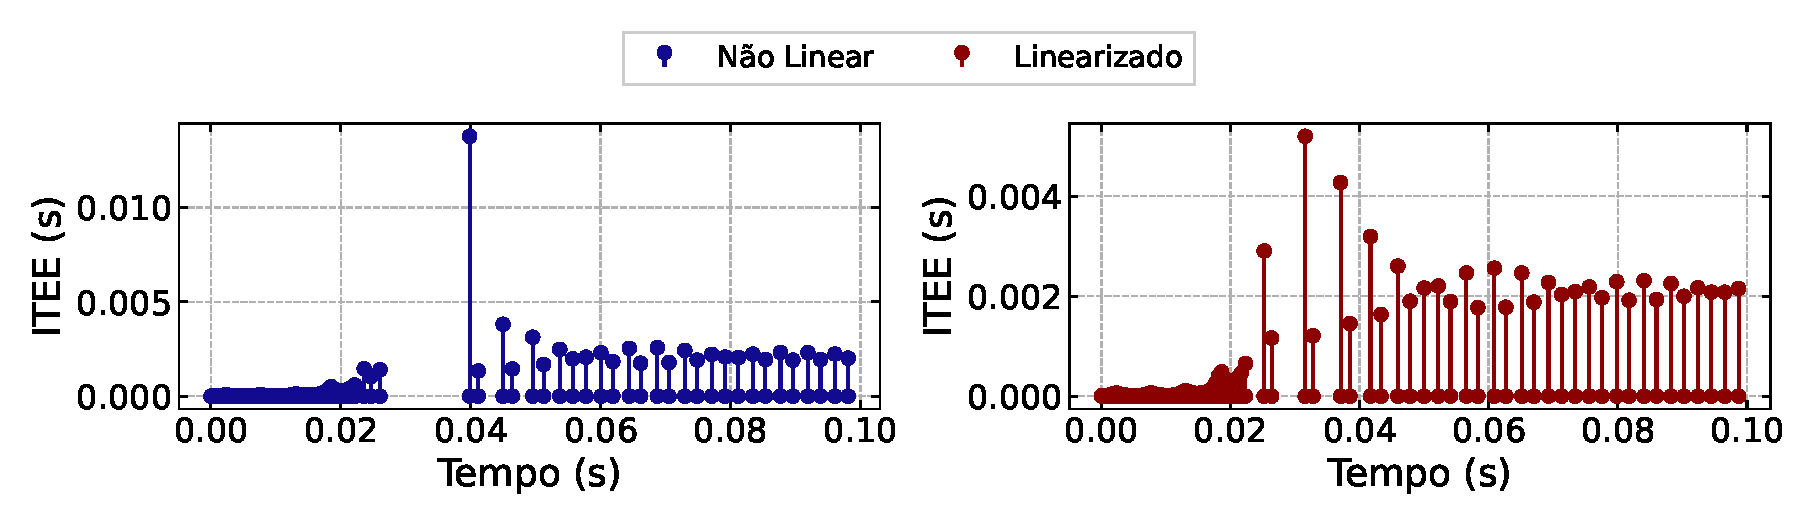
\includegraphics[width=1.\textwidth]{figuras/dynamic-etm/buck/sim1/op2/inter-event-times.eps}
  \caption{Tempo entre evento do conversor Buck em torno do ponto de operação $P_{\mathrm{o}, 2}$ sob sinal de pertubação $P_{\mathrm{cpl}}(t)$ constante e \acrshort{etm} estático.}
  % \label{fig:simulation_2_boost_op2}
\end{figure}

\begin{figure}[H]
  \centering
  \captionsetup{justification=centering}
  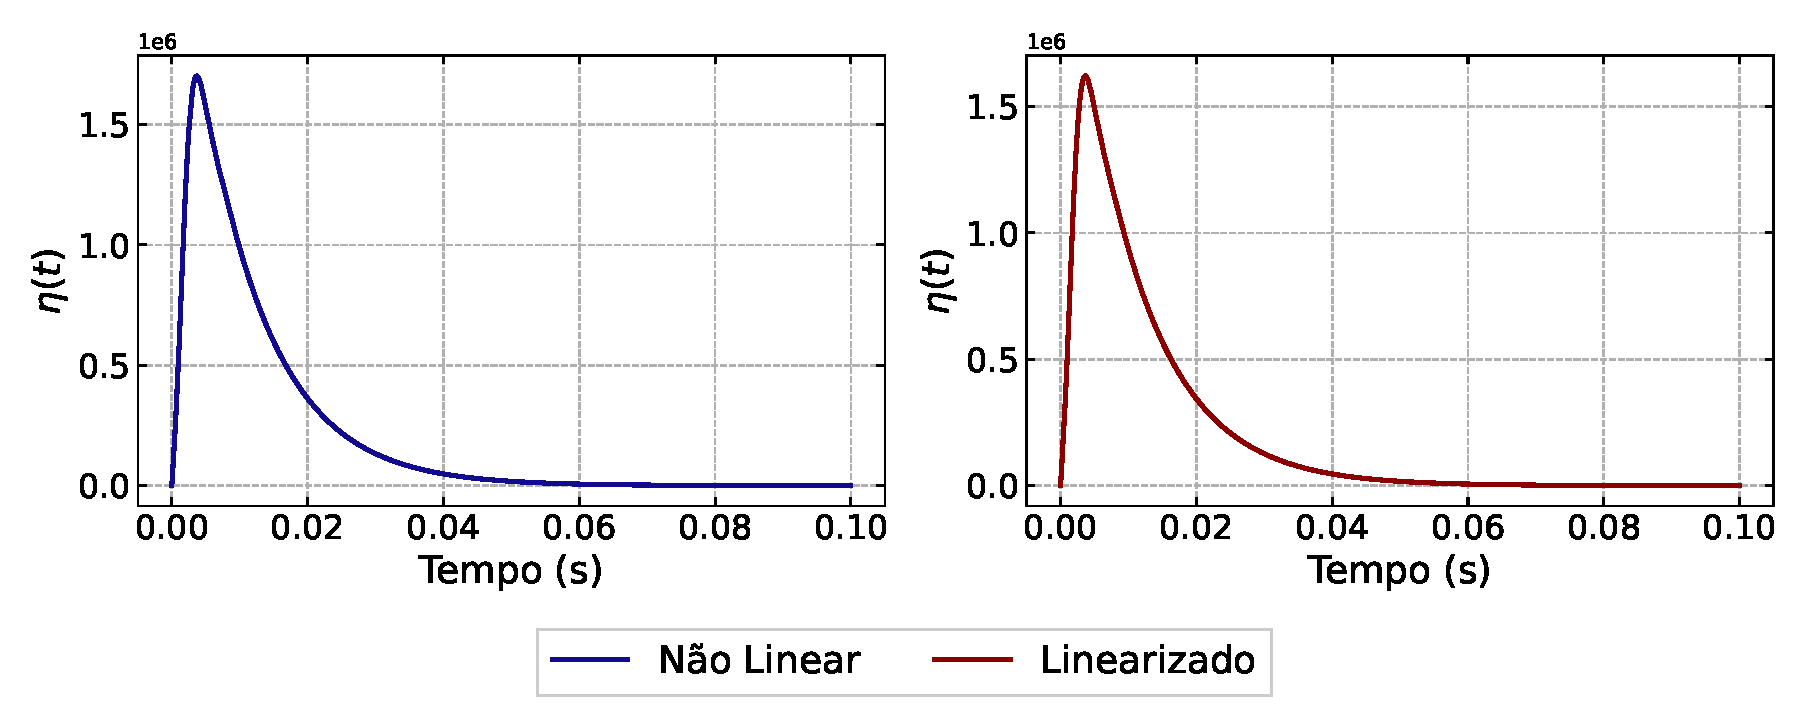
\includegraphics[width=1.\textwidth]{figuras/dynamic-etm/buck/sim1/op2/eta.eps}
  \caption{Variável dinâmica $\eta(t)$ do \acrshort{etm} dinâmico na simulação do conversor Buck em torno do ponto de operação $P_{\mathrm{o}, 2}$ sob sinal de pertubação $P_{\mathrm{cpl}}(t)$ constante.}
  % \label{fig:simulation_2_boost_op2}
\end{figure}

\subsubsection{Sinal de Pertubação Variável}

\begin{figure}[H]
  \centering
  \captionsetup{justification=centering}
  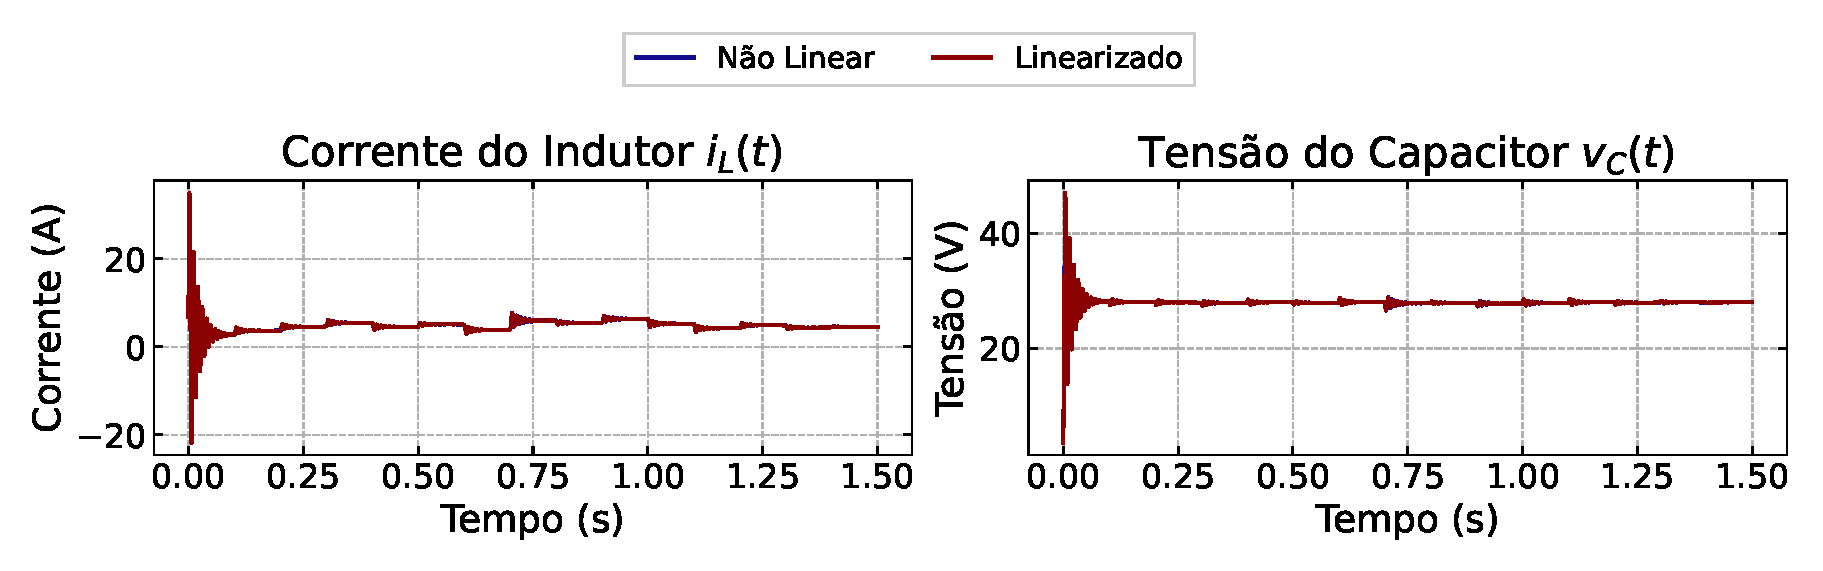
\includegraphics[width=1.\textwidth]{figuras/dynamic-etm/buck/sim2/op1/result.eps}
  \caption{Estados do conversor Buck em torno do ponto de operação $P_{\mathrm{o}, 1}$ sob sinal de pertubação $P_{\mathrm{cpl}}(t)$ variável e \acrshort{etm} estático.}
  % \label{fig:simulation_2_boost_op2}
\end{figure}

\begin{figure}[H]
  \centering
  \captionsetup{justification=centering}
  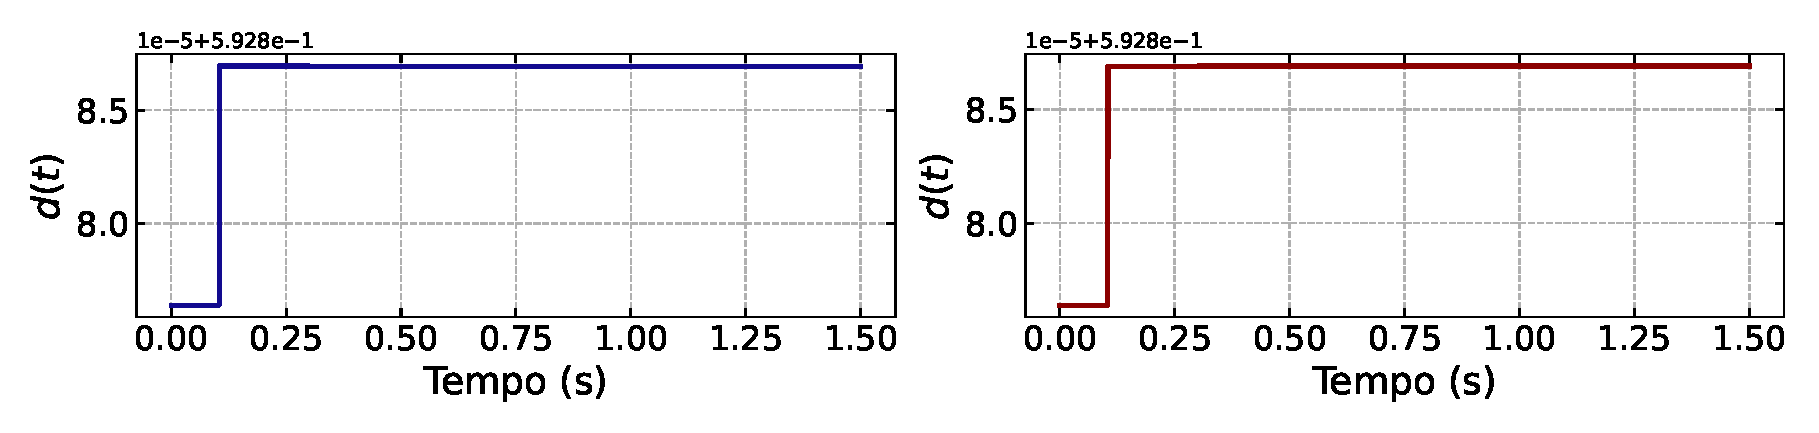
\includegraphics[width=1.\textwidth]{figuras/dynamic-etm/buck/sim2/op1/duty-cycle.eps}
  \caption{Entrada duty cycle $d(t)$ do conversor Buck em torno do ponto de operação $P_{\mathrm{o}, 1}$ sob sinal de pertubação $P_{\mathrm{cpl}}(t)$ variável e \acrshort{etm} estático.}
  % \label{fig:simulation_2_boost_op2}
\end{figure}

\begin{figure}[H]
  \centering
  \captionsetup{justification=centering}
  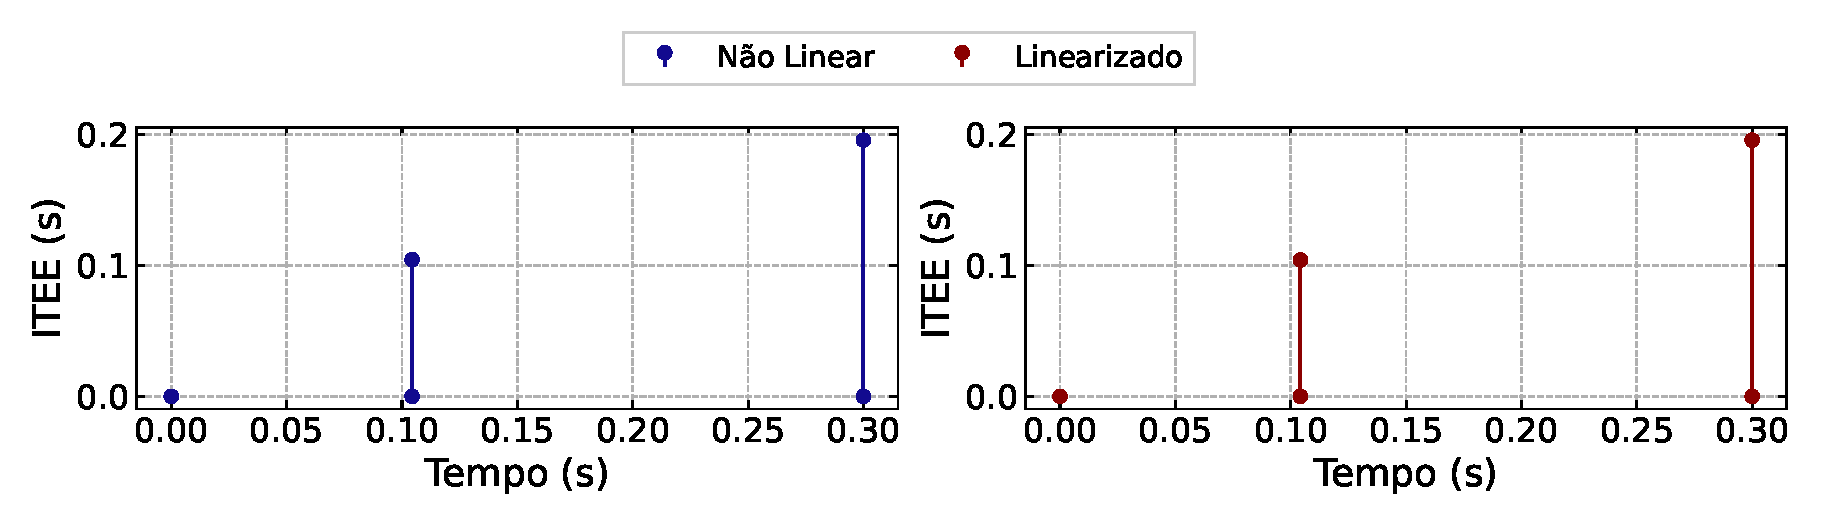
\includegraphics[width=1.\textwidth]{figuras/dynamic-etm/buck/sim2/op1/inter-event-times.eps}
  \caption{Tempo entre evento do conversor Buck em torno do ponto de operação $P_{\mathrm{o}, 1}$ sob sinal de pertubação $P_{\mathrm{cpl}}(t)$ variável e \acrshort{etm} estático.}
  % \label{fig:simulation_2_boost_op2}
\end{figure}

\begin{figure}[H]
  \centering
  \captionsetup{justification=centering}
  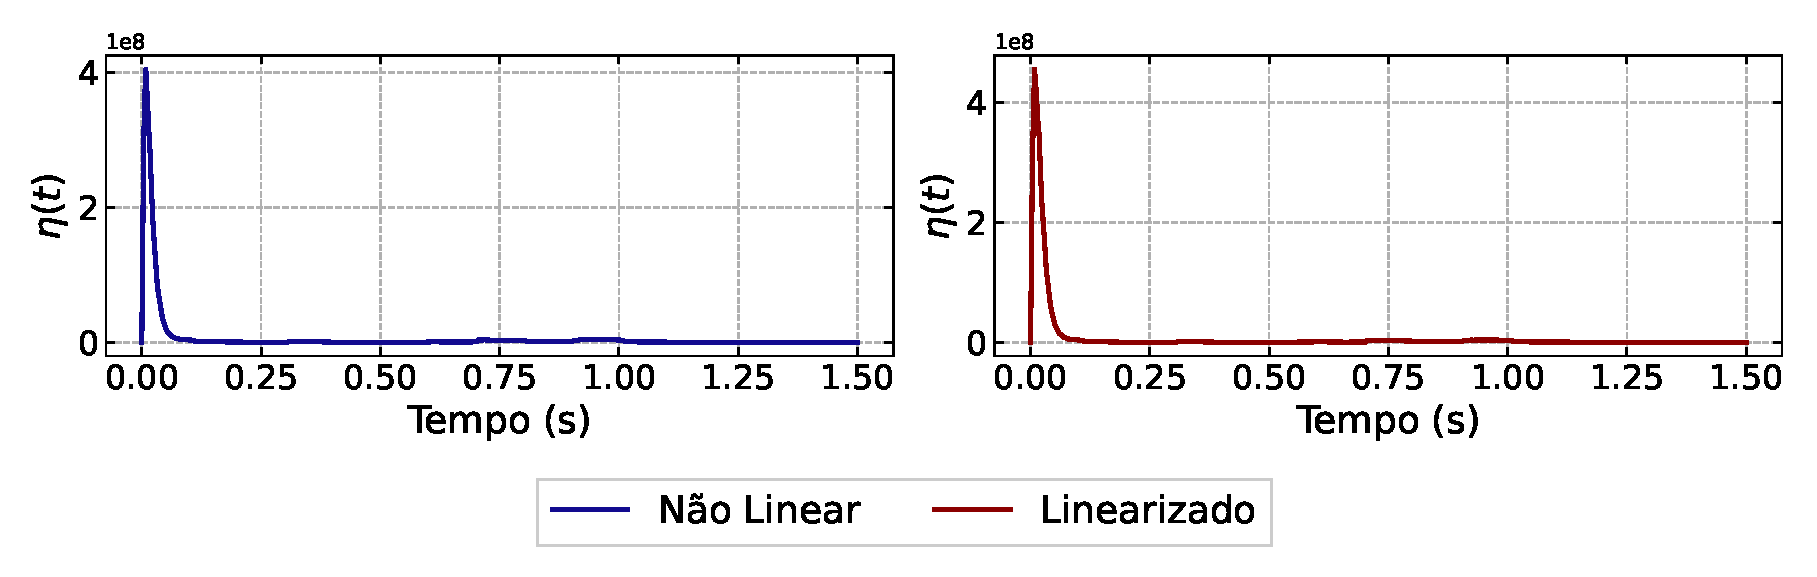
\includegraphics[width=1.\textwidth]{figuras/dynamic-etm/buck/sim2/op1/eta.eps}
  \caption{Variável dinâmica $\eta(t)$ do \acrshort{etm} dinâmico na simulação do conversor Buck em torno do ponto de operação $P_{\mathrm{o}, 2}$ sob sinal de pertubação $P_{\mathrm{cpl}}(t)$ constante.}
  % \label{fig:simulation_2_boost_op2}
\end{figure}

% Instável

\begin{figure}[H]
  \centering
  \captionsetup{justification=centering}
  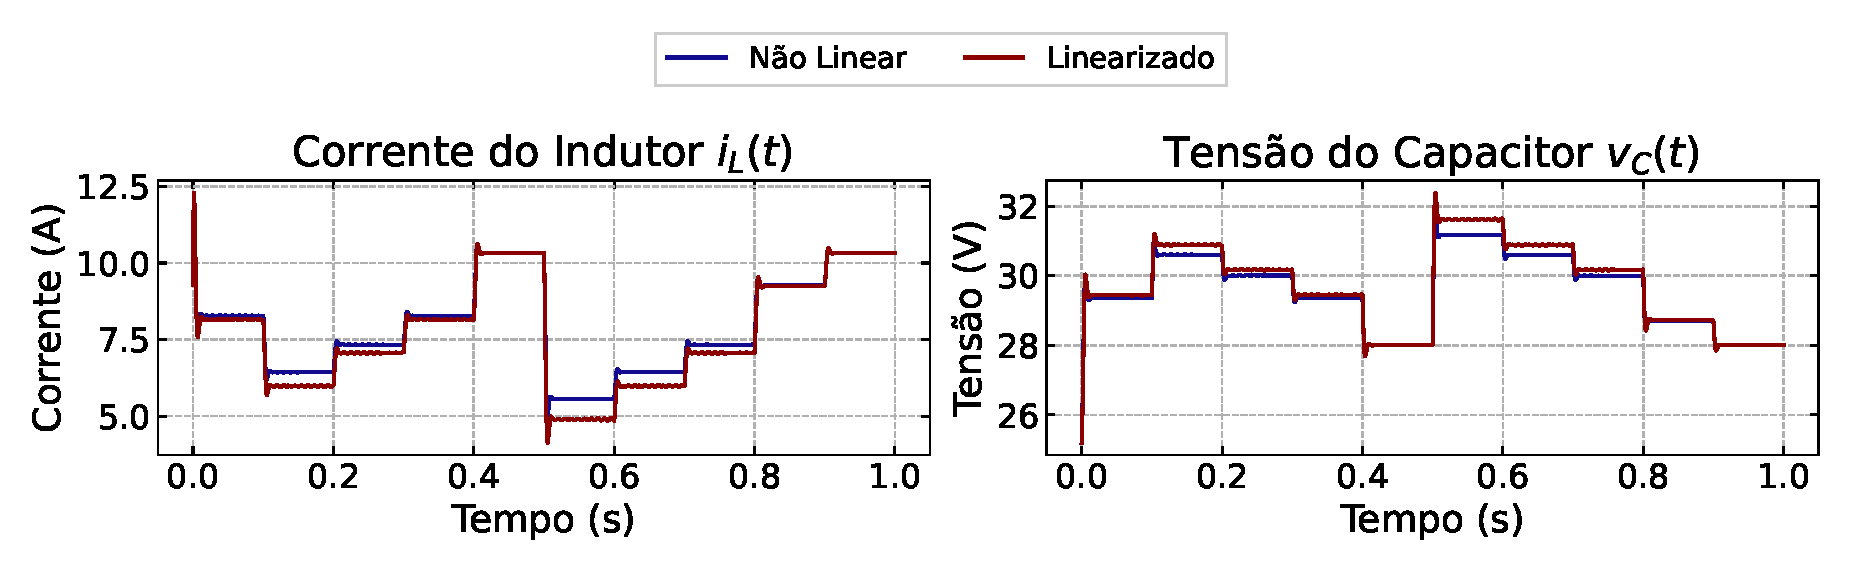
\includegraphics[width=1.\textwidth]{figuras/dynamic-etm/buck/sim2/op2/result.eps}
  \caption{Estados do conversor Buck em torno do ponto de operação $P_{\mathrm{o}, 2}$ sob sinal de pertubação $P_{\mathrm{cpl}}(t)$ variável e \acrshort{etm} estático.}
  % \label{fig:simulation_2_boost_op2}
\end{figure}

\begin{figure}[H]
  \centering
  \captionsetup{justification=centering}
  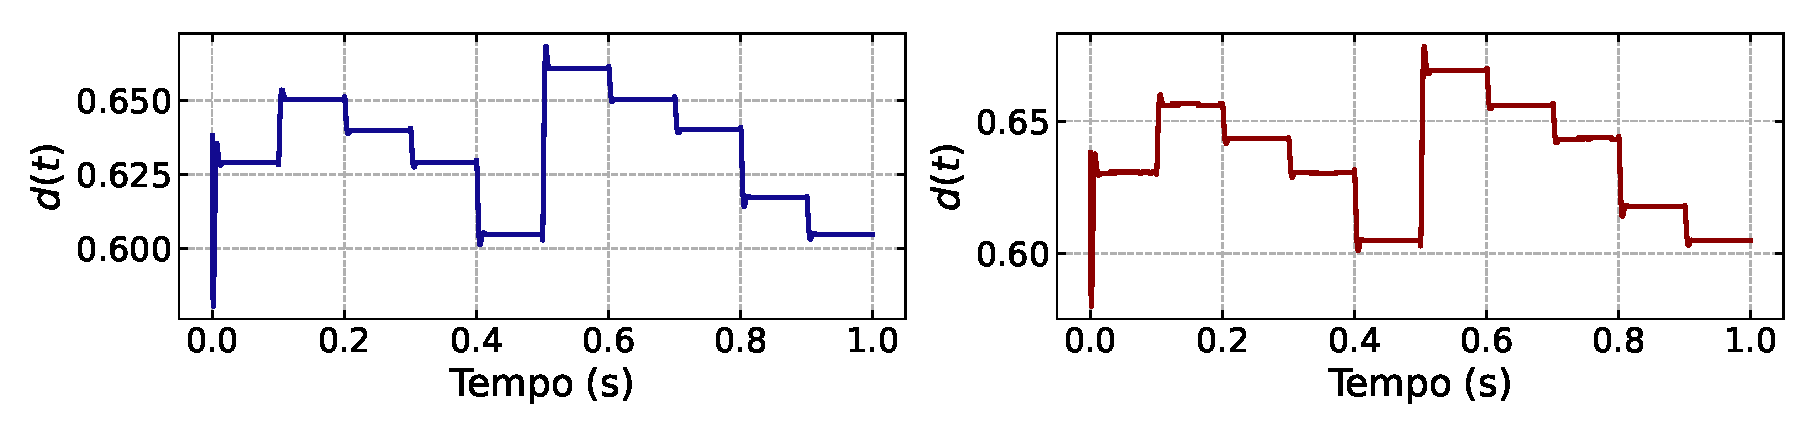
\includegraphics[width=1.\textwidth]{figuras/dynamic-etm/buck/sim2/op2/duty-cycle.eps}
  \caption{Entrada duty cycle $d(t)$ do conversor Buck em torno do ponto de operação $P_{\mathrm{o}, 2}$ sob sinal de pertubação $P_{\mathrm{cpl}}(t)$ variável e \acrshort{etm} estático.}
  % \label{fig:simulation_2_boost_op2}
\end{figure}

\begin{figure}[H]
  \centering
  \captionsetup{justification=centering}
  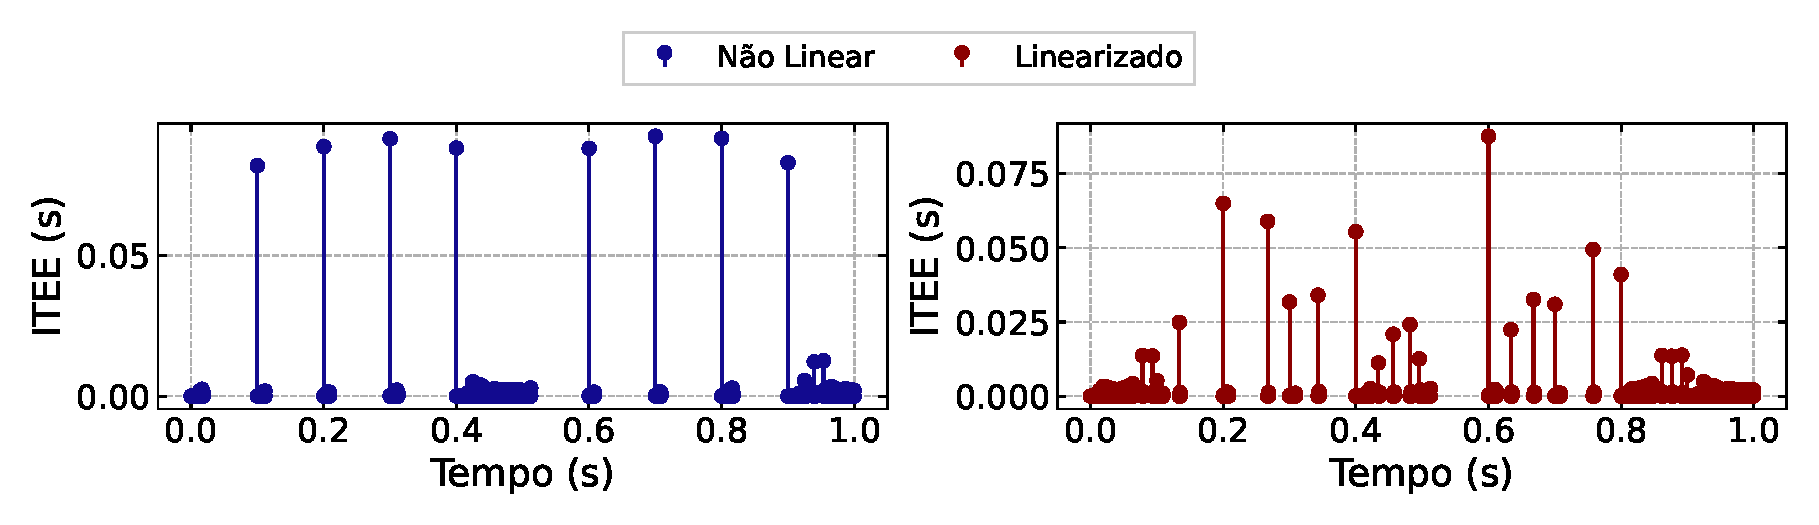
\includegraphics[width=1.\textwidth]{figuras/dynamic-etm/buck/sim2/op2/inter-event-times.eps}
  \caption{Tempo entre evento do conversor Buck em torno do ponto de operação $P_{\mathrm{o}, 2}$ sob sinal de pertubação $P_{\mathrm{cpl}}(t)$ variável e \acrshort{etm} estático.}
  % \label{fig:simulation_2_boost_op2}
\end{figure}

\begin{figure}[H]
  \centering
  \captionsetup{justification=centering}
  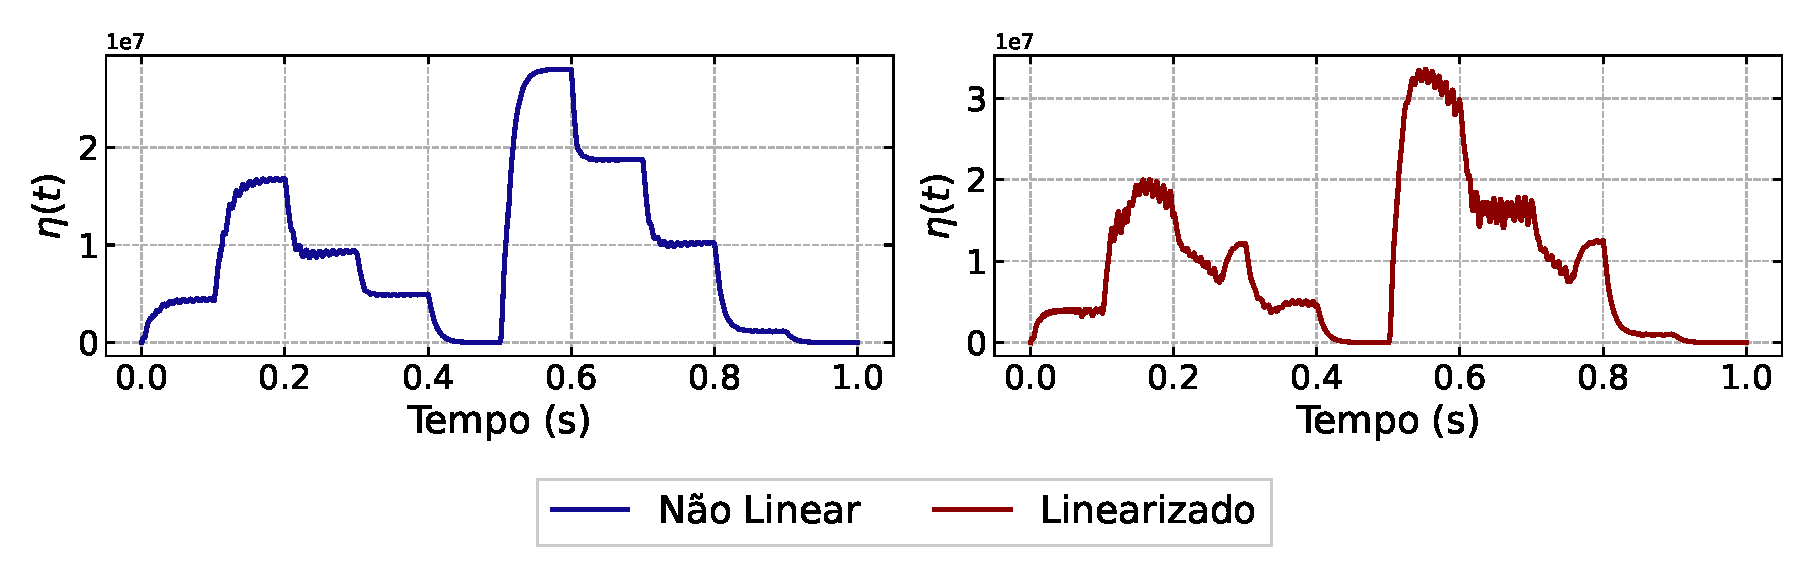
\includegraphics[width=1.\textwidth]{figuras/dynamic-etm/buck/sim2/op2/eta.eps}
  \caption{Variável dinâmica $\eta(t)$ do \acrshort{etm} dinâmico na simulação do conversor Buck em torno do ponto de operação $P_{\mathrm{o}, 2}$ sob sinal de pertubação $P_{\mathrm{cpl}}(t)$ constante.}
  % \label{fig:simulation_2_boost_op2}
\end{figure}

\subsection{Conversor Boost}
\subsubsection{Sinal de Pertubação Constante}

\begin{figure}[H]
  \centering
  \captionsetup{justification=centering}
  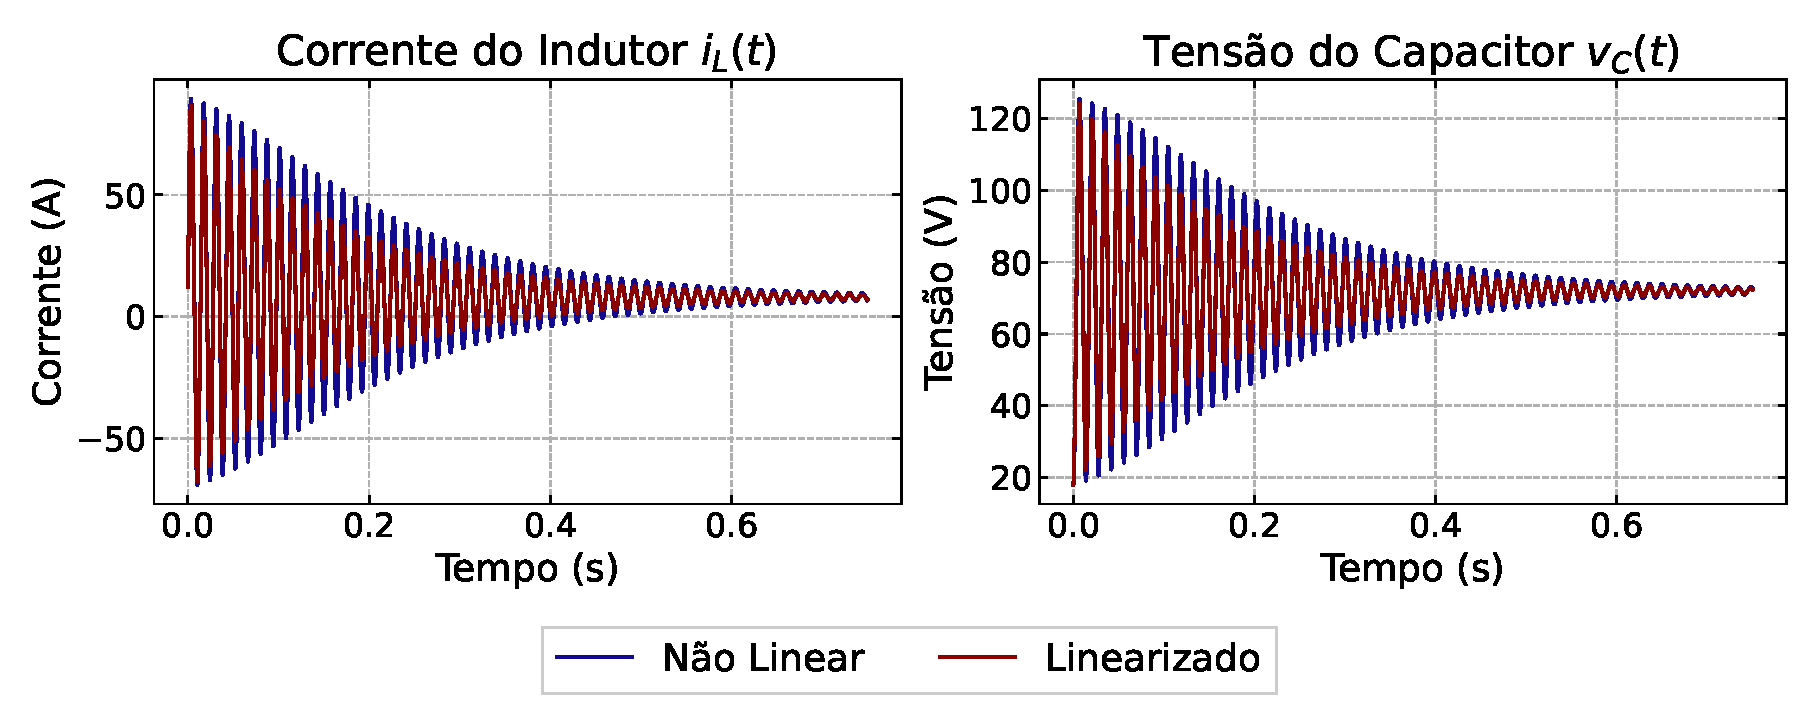
\includegraphics[width=1.\textwidth]{figuras/dynamic-etm/boost/sim1/op1/result.eps}
  \caption{Estados do conversor Boost em torno do ponto de operação $P_{\mathrm{o}, 3}$ sob sinal de pertubação $P_{\mathrm{cpl}}(t)$ constante e \acrshort{etm} estático.}
  % \label{fig:simulation_2_boost_op2}
\end{figure}

\begin{figure}[H]
  \centering
  \captionsetup{justification=centering}
  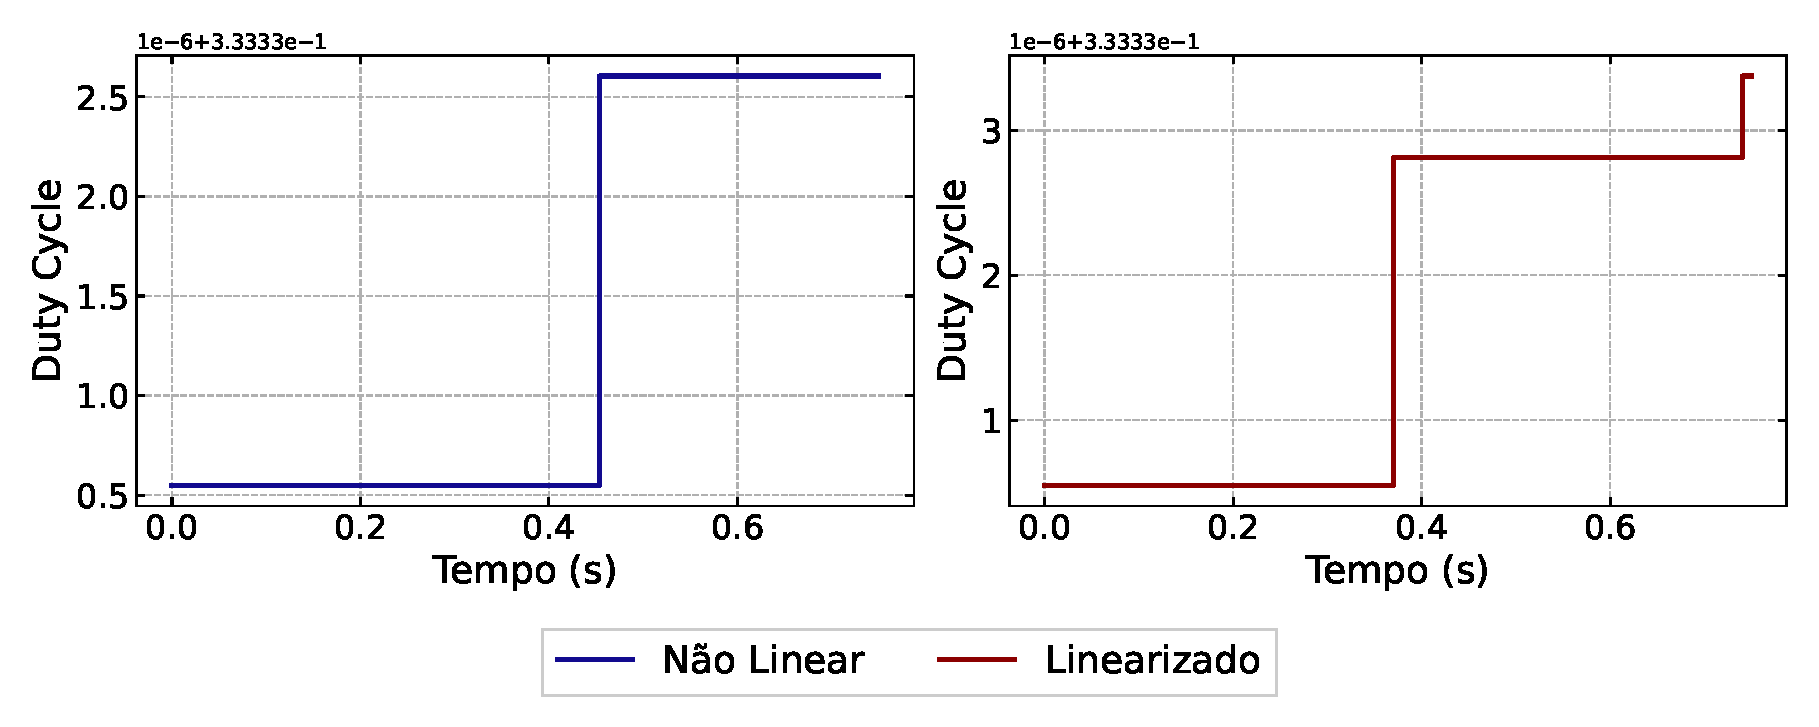
\includegraphics[width=1.\textwidth]{figuras/dynamic-etm/boost/sim1/op1/duty-cycle.eps}
  \caption{Entrada duty cycle $d(t)$ do conversor Boost em torno do ponto de operação $P_{\mathrm{o}, 3}$ sob sinal de pertubação $P_{\mathrm{cpl}}(t)$ constante e \acrshort{etm} estático.}
  % \label{fig:simulation_2_boost_op2}
\end{figure}

\begin{figure}[H]
  \centering
  \captionsetup{justification=centering}
  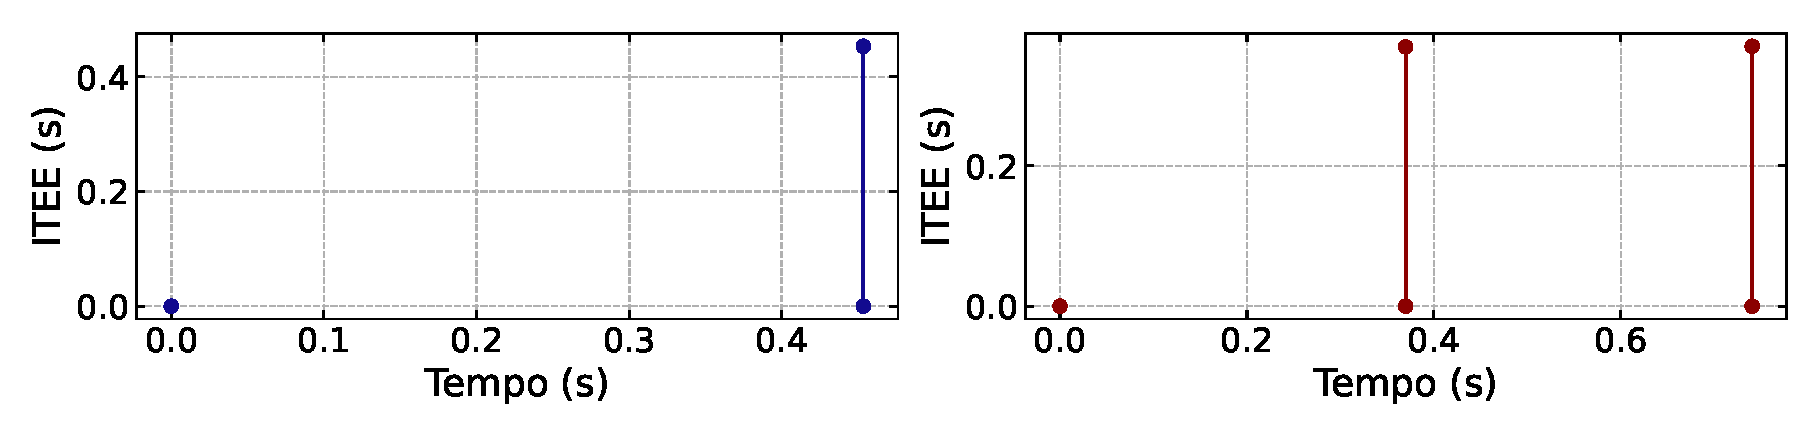
\includegraphics[width=1.\textwidth]{figuras/dynamic-etm/boost/sim1/op1/inter-event-times.eps}
  \caption{Tempo entre evento do conversor Boost em torno do ponto de operação $P_{\mathrm{o}, 3}$ sob sinal de pertubação $P_{\mathrm{cpl}}(t)$ constante e \acrshort{etm} estático.}
  % \label{fig:simulation_2_boost_op2}
\end{figure}

\begin{figure}[H]
  \centering
  \captionsetup{justification=centering}
  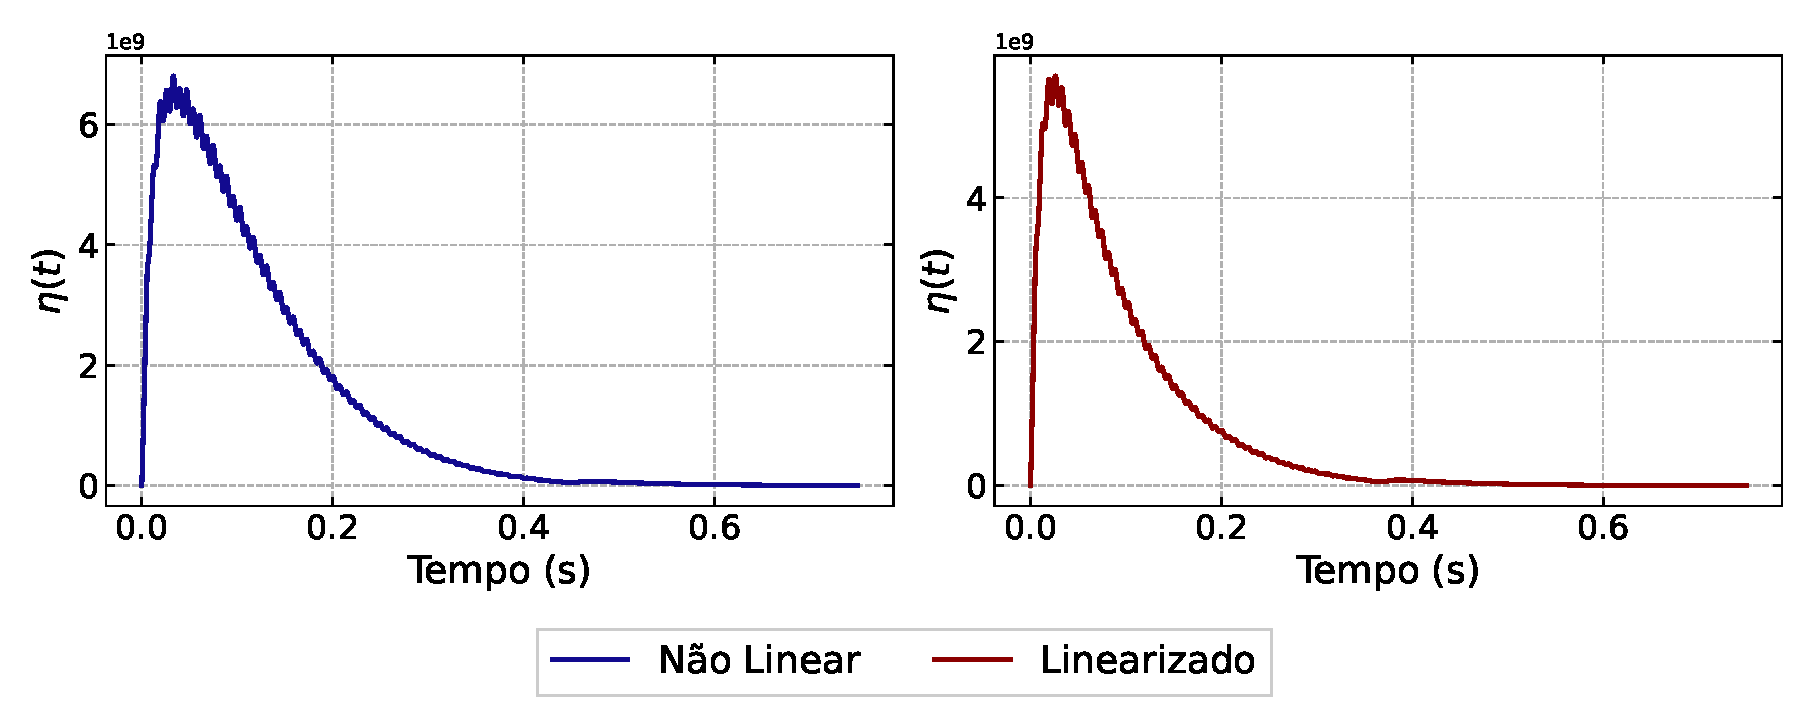
\includegraphics[width=1.\textwidth]{figuras/dynamic-etm/boost/sim1/op1/eta.eps}
  \caption{Variável dinâmica $\eta(t)$ do \acrshort{etm} dinâmico na simulação do conversor Boost em torno do ponto de operação $P_{\mathrm{o}, 3}$ sob sinal de pertubação $P_{\mathrm{cpl}}(t)$ constante.}
  % \label{fig:simulation_2_boost_op2}
\end{figure}

\begin{figure}[H]
  \centering
  \captionsetup{justification=centering}
  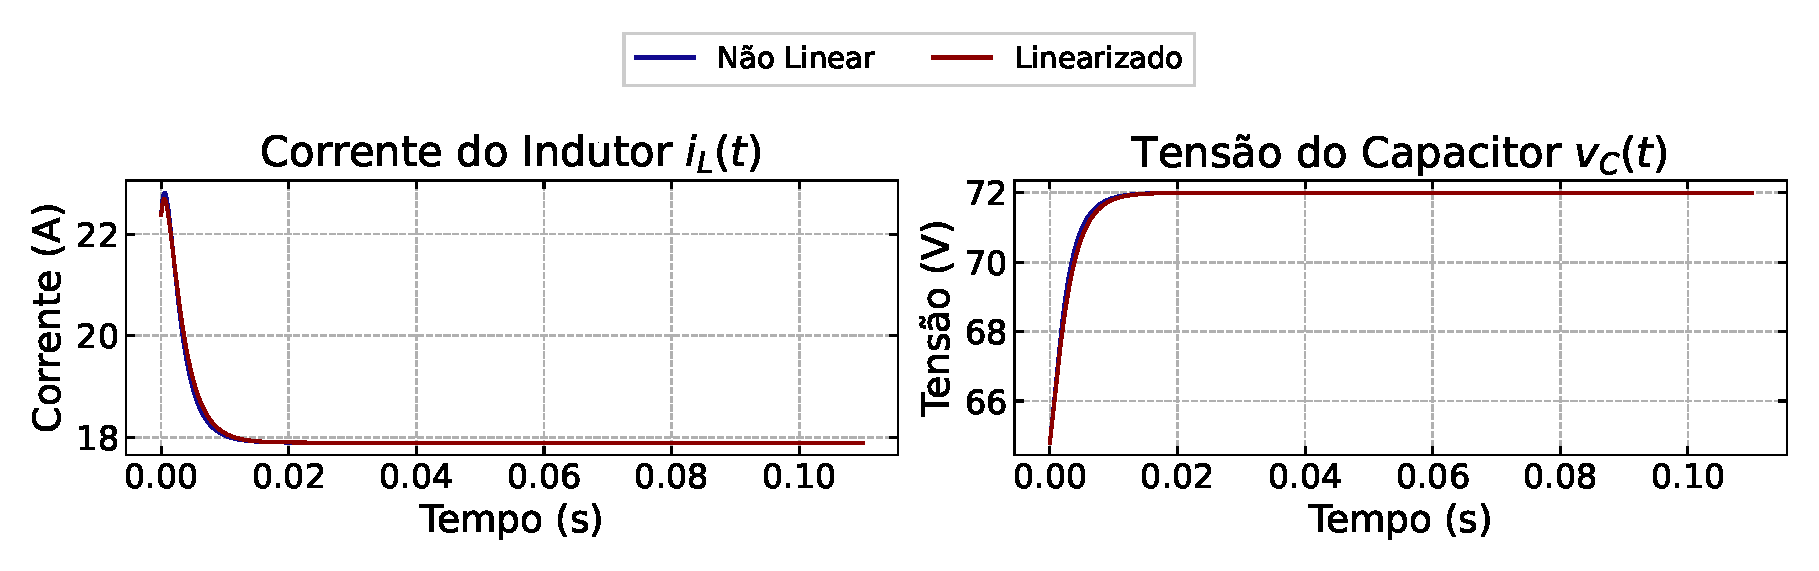
\includegraphics[width=1.\textwidth]{figuras/dynamic-etm/boost/sim1/op2/result.eps}
  \caption{Estados do conversor Boost em torno do ponto de operação $P_{\mathrm{o}, 4}$ sob sinal de pertubação $P_{\mathrm{cpl}}(t)$ constante e \acrshort{etm} estático.}
  % \label{fig:simulation_2_boost_op2}
\end{figure}

\begin{figure}[H]
  \centering
  \captionsetup{justification=centering}
  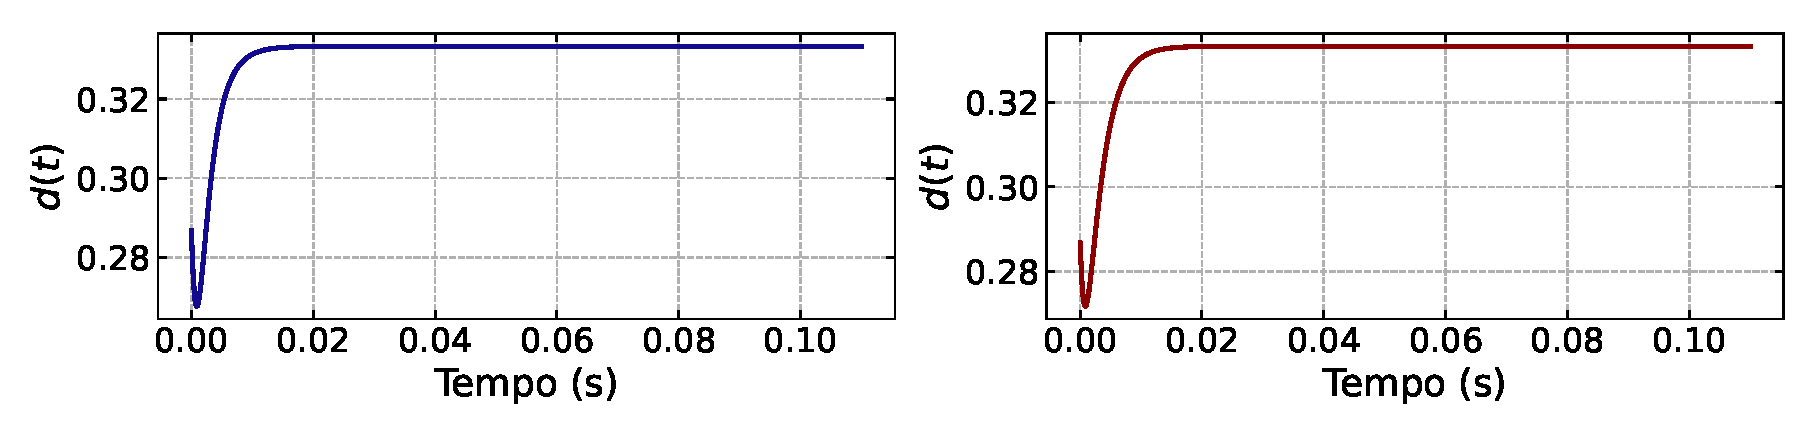
\includegraphics[width=1.\textwidth]{figuras/dynamic-etm/boost/sim1/op2/duty-cycle.eps}
  \caption{Entrada duty cycle $d(t)$ do conversor Boost em torno do ponto de operação $P_{\mathrm{o}, 4}$ sob sinal de pertubação $P_{\mathrm{cpl}}(t)$ constante e \acrshort{etm} estático.}
  % \label{fig:simulation_2_boost_op2}
\end{figure}

\begin{figure}[H]
  \centering
  \captionsetup{justification=centering}
  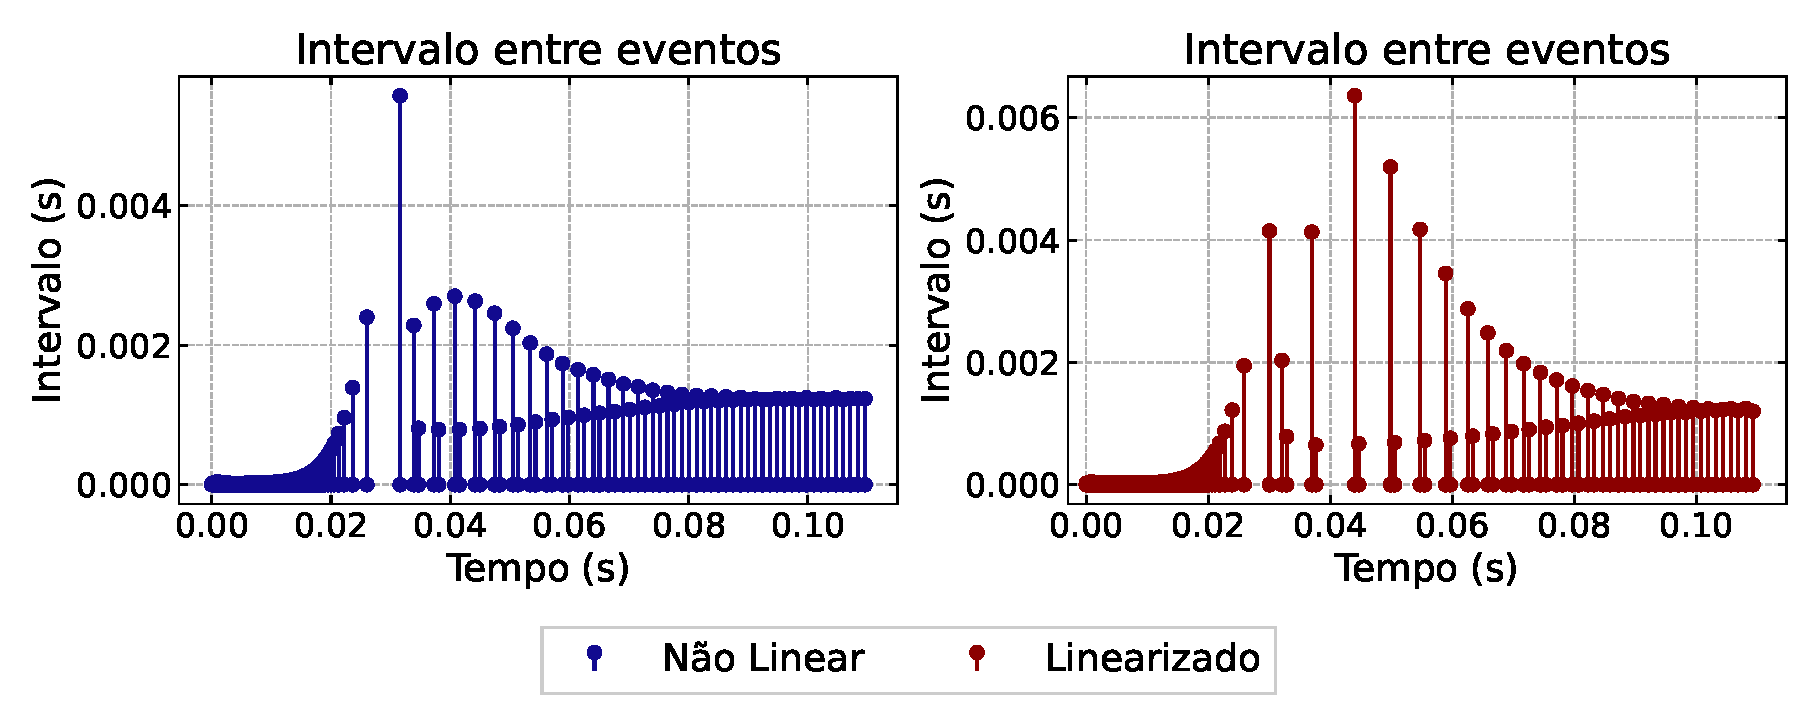
\includegraphics[width=1.\textwidth]{figuras/dynamic-etm/boost/sim1/op2/inter-event-times.eps}
  \caption{Tempo entre evento do conversor Boost em torno do ponto de operação $P_{\mathrm{o}, 4}$ sob sinal de pertubação $P_{\mathrm{cpl}}(t)$ constante e \acrshort{etm} estático.}
  % \label{fig:simulation_2_boost_op2}
\end{figure}

\begin{figure}[H]
  \centering
  \captionsetup{justification=centering}
  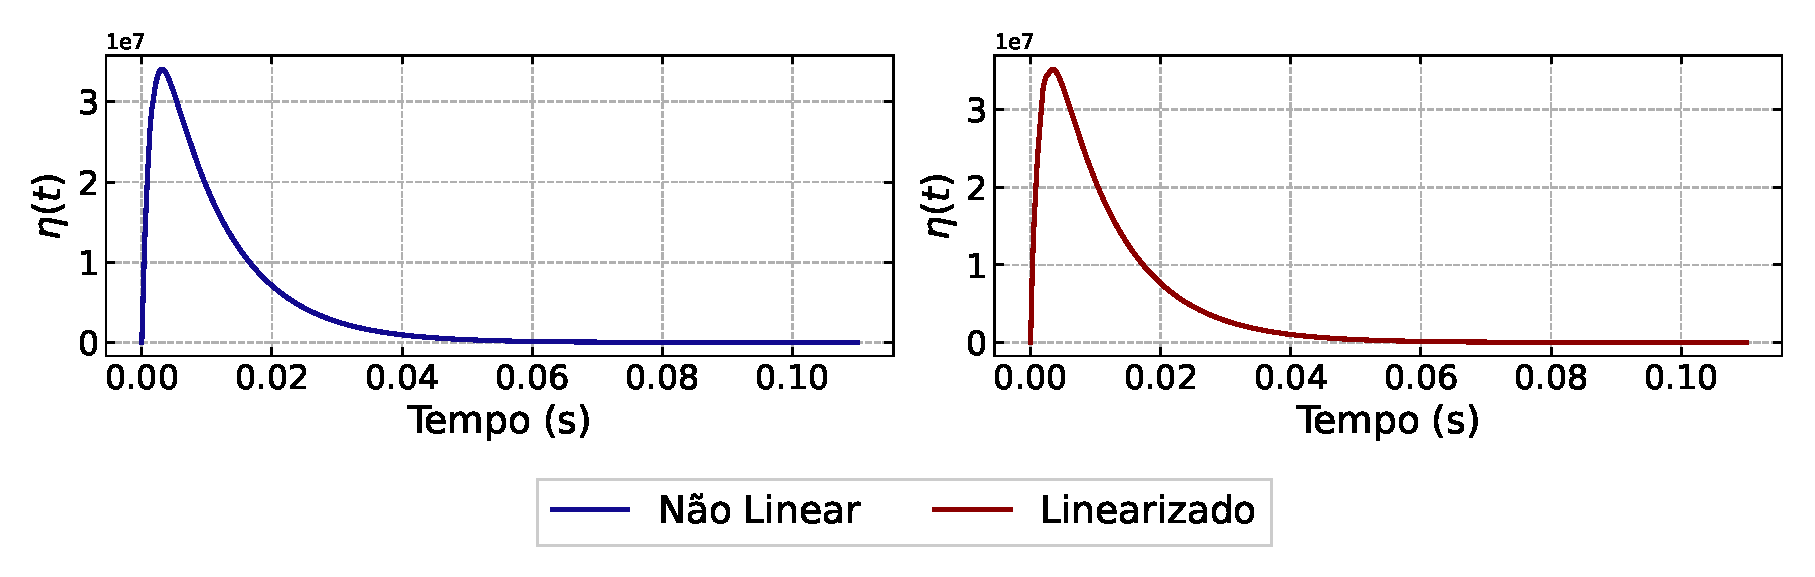
\includegraphics[width=1.\textwidth]{figuras/dynamic-etm/boost/sim1/op2/eta.eps}
  \caption{Variável dinâmica $\eta(t)$ do \acrshort{etm} dinâmico na simulação do conversor Buck em torno do ponto de operação $P_{\mathrm{o}, 4}$ sob sinal de pertubação $P_{\mathrm{cpl}}(t)$ constante.}
  % \label{fig:simulation_2_boost_op2}
\end{figure}

\subsubsection{Sinal de Pertubação Variável}

\begin{figure}[H]
  \centering
  \captionsetup{justification=centering}
  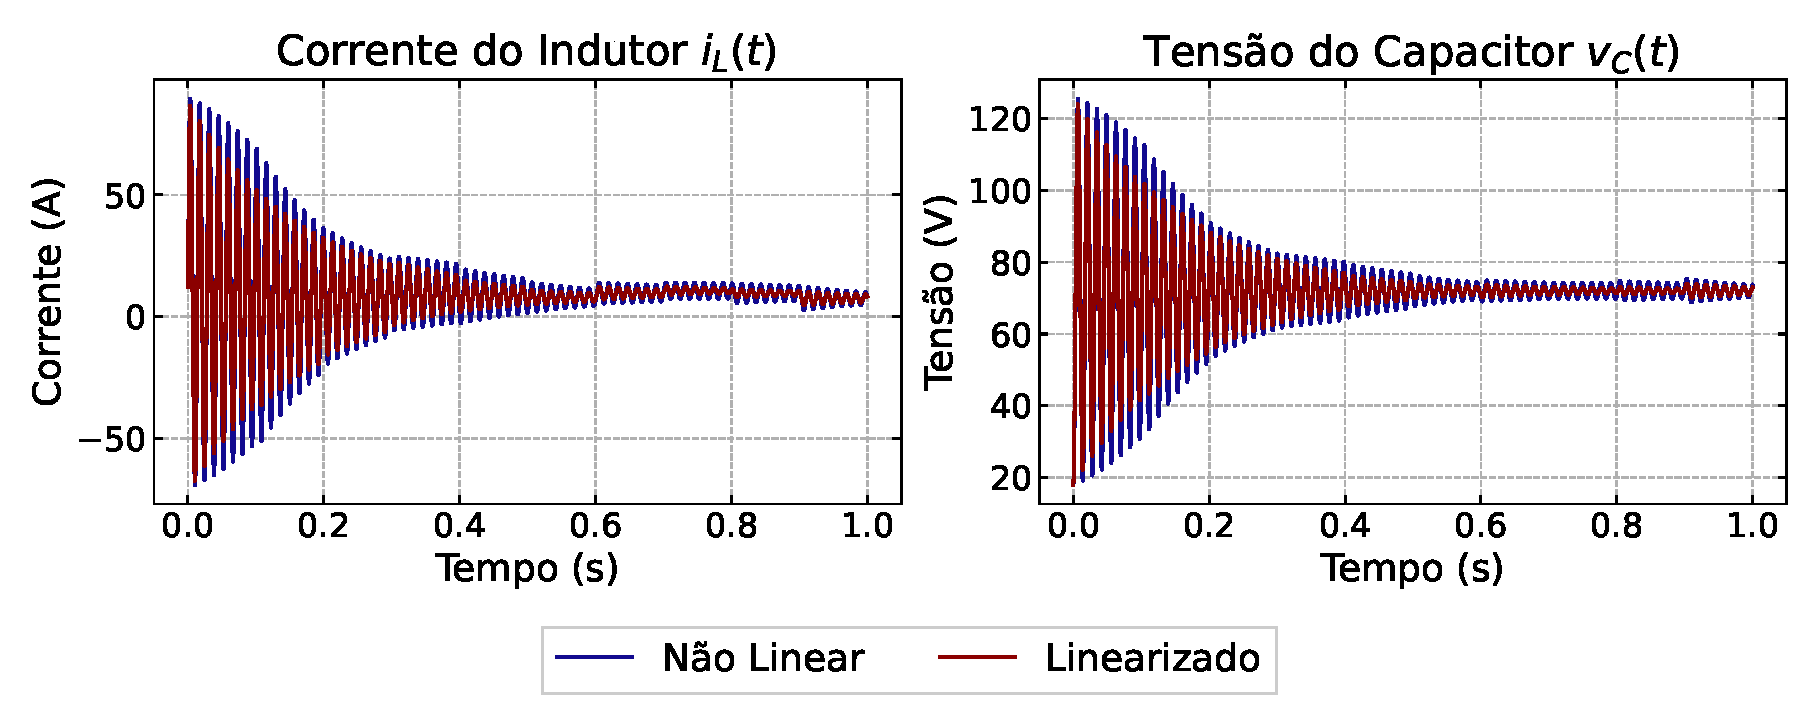
\includegraphics[width=1.\textwidth]{figuras/dynamic-etm/boost/sim2/op1/result.eps}
  \caption{Estados do conversor Boost em torno do ponto de operação $P_{\mathrm{o}, 3}$ sob sinal de pertubação $P_{\mathrm{cpl}}(t)$ variável e \acrshort{etm} estático.}
  % \label{fig:simulation_2_boost_op2}
\end{figure}

\begin{figure}[H]
  \centering
  \captionsetup{justification=centering}
  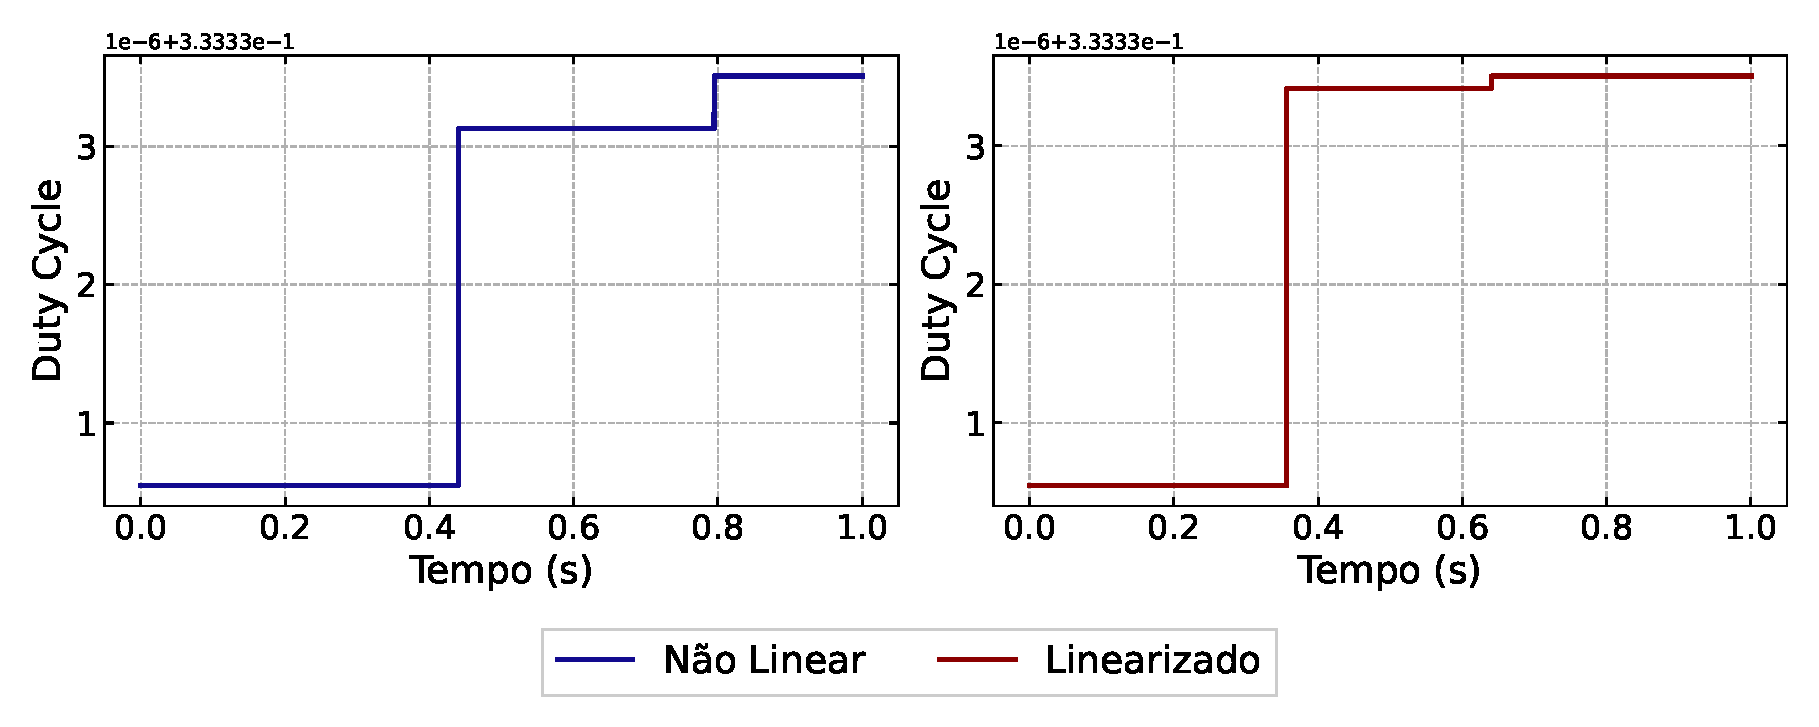
\includegraphics[width=1.\textwidth]{figuras/dynamic-etm/boost/sim2/op1/duty-cycle.eps}
  \caption{Entrada duty cycle $d(t)$ do conversor Boost em torno do ponto de operação $P_{\mathrm{o}, 3}$ sob sinal de pertubação $P_{\mathrm{cpl}}(t)$ variável e \acrshort{etm} estático.}
  % \label{fig:simulation_2_boost_op2}
\end{figure}

\begin{figure}[H]
  \centering
  \captionsetup{justification=centering}
  \includegraphics[width=1.\textwidth]{figuras/dynamic-etm/boost/sim2/op1/inter-event-times.eps}
  \caption{Tempo entre evento do conversor Boost em torno do ponto de operação $P_{\mathrm{o}, 3}$ sob sinal de pertubação $P_{\mathrm{cpl}}(t)$ variável e \acrshort{etm} estático.}
  % \label{fig:simulation_2_boost_op2}
\end{figure}

\begin{figure}[H]
  \centering
  \captionsetup{justification=centering}
  \includegraphics[width=1.\textwidth]{figuras/dynamic-etm/boost/sim2/op1/eta.eps}
  \caption{Variável dinâmica $\eta(t)$ do \acrshort{etm} dinâmico na simulação do conversor Buck em torno do ponto de operação $P_{\mathrm{o}, 3}$ sob sinal de pertubação $P_{\mathrm{cpl}}(t)$ variável.}
  % \label{fig:simulation_2_boost_op2}
\end{figure}

\begin{figure}[H]
  \centering
  \captionsetup{justification=centering}
  \includegraphics[width=1.\textwidth]{figuras/dynamic-etm/boost/sim2/op2/result.eps}
  \caption{Estados do conversor Boost em torno do ponto de operação $P_{\mathrm{o}, 4}$ sob sinal de pertubação $P_{\mathrm{cpl}}(t)$ variável e \acrshort{etm} estático.}
  % \label{fig:simulation_2_boost_op2}
\end{figure}

\begin{figure}[H]
  \centering
  \captionsetup{justification=centering}
  \includegraphics[width=1.\textwidth]{figuras/dynamic-etm/boost/sim2/op2/duty-cycle.eps}
  \caption{Entrada duty cycle $d(t)$ do conversor Boost em torno do ponto de operação $P_{\mathrm{o}, 4}$ sob sinal de pertubação $P_{\mathrm{cpl}}(t)$ variável e \acrshort{etm} estático.}
  % \label{fig:simulation_2_boost_op2}
\end{figure}

\begin{figure}[H]
  \centering
  \captionsetup{justification=centering}
  \includegraphics[width=1.\textwidth]{figuras/dynamic-etm/boost/sim2/op2/inter-event-times.eps}
  \caption{Tempo entre evento do conversor Boost em torno do ponto de operação $P_{\mathrm{o}, 4}$ sob sinal de pertubação $P_{\mathrm{cpl}}(t)$ variável e \acrshort{etm} estático.}
  % \label{fig:simulation_2_boost_op2}
\end{figure}

\begin{figure}[H]
  \centering
  \captionsetup{justification=centering}
  \includegraphics[width=1.\textwidth]{figuras/dynamic-etm/boost/sim2/op2/eta.eps}
  \caption{Variável dinâmica $\eta(t)$ do \acrshort{etm} dinâmico na simulação do conversor Buck em torno do ponto de operação $P_{\mathrm{o}, 4}$ sob sinal de pertubação $P_{\mathrm{cpl}}(t)$ variável.}
  % \label{fig:simulation_2_boost_op2}
\end{figure}